\documentclass[a4paper]{book}
\usepackage[utf8]{inputenc}
\usepackage[margin=3cm]{geometry} % For smaller margins
\usepackage{appendix} % For appendix support
\usepackage{tikz, pgfplots} % For the skill outcome graph
    \pgfplotsset{width = \textwidth, compat = newest}
\usepackage{graphicx} % For advanced picture insertion
\usepackage{pdfpages} % For inserting PDFs
\usepackage{multicol} % For supporting multi-columnar tables
\usepackage{tcolorbox} % For coloured info boxes
    \tcbuselibrary{skins}
    \tcbset{colback=brown!10, fonttitle=\scshape}
\usepackage{textcomp} % For the interrobang
\usepackage[sc,sf,bf]{titlesec} % for custom titles
\usepackage{sectsty} % for section styles
\usepackage{fancyhdr} % for "fancy" headers
\usepackage[notmath]{sansmathfonts} % for a sans-serif small-caps font
\usepackage{enumitem} % for finer control over enumerations
 
%%%%%%%%%%%%%%%%%%%%%%%%%%%%%%%%%
%% CHAPTERS & SECTION HEADINGS %%
%%%%%%%%%%%%%%%%%%%%%%%%%%%%%%%%%


% Simplifies chapter titles
% No longer says
% Chapter 2
% Game Creation
% but instead simply
% 2 Game Creation
\titleformat{\chapter}[hang]
{\sffamily\bfseries\scshape\Huge}
{\thechapter\quad}{0pt}{}{}

% Removes unnecessarily large margin above chapter title
\titlespacing*{\chapter}{0pt}{-\topskip}{40pt}

% Set the remaining titles to be sans serif and small caps
\allsectionsfont{\sffamily\scshape}

%%%%%%%%%%%%%%%%%
%% THUMB INDEX %%
%%%%%%%%%%%%%%%%%

\renewcommand{\chaptermark}[1]{\markboth{\textsc{\thechapter\ #1}}{}}

%%%%%%%%%%%%%%%%%%%%%%%
%% CUSTOM TEXT BOXES %%
%%%%%%%%%%%%%%%%%%%%%%%
\newtcolorbox{note}{
    enhanced, % enable advanced settings
    left = 10mm, % pushes text away from the left edge by 10mm
    sharp corners, % disables rounded corners
    rounded corners = southeast, % "round" the bottom right corner
    arc is angular, % make the "round" corner an angle
    arc = 3mm, % controls corner cut
    boxrule=0.6pt, % sets box line thickness
    underlay={%
        \path[fill=tcbcolback!80!black] ([yshift=3mm]interior.south east)--++(-0.4,-0.1)--++(0.1,-0.2); % triangle
        \path[draw=tcbcolframe,shorten <=-0.05mm,shorten >=-0.05mm] ([yshift=3mm]interior.south east)--++(-0.4,-0.1)--++(0.1,-0.2); % triangle edge
        \path[fill=gray!50!black,draw=none] (interior.south west) rectangle node[brown!10]{\Huge\bfseries \textinterrobang} ([xshift=8mm]interior.north west);
    },
    drop fuzzy shadow % adds drop shadow
}

\newtcolorbox{example}{
    enhanced,
    title = Example,
    before upper={\parindent15pt\noindent} % add paragraph indentation
}

\begin{document}

\begin{titlepage}
\begin{center}
  \includegraphics[width = \textwidth]{graphics/svg-logo.png}
  \LARGE{$\beta2.0.0$ --- By Niko Lepka}\\
  \Large{\today}
\end{center}
\end{titlepage}
\thispagestyle{empty} % removes page number from front page
\frontmatter % adds Roman numerals to the preface chapter
\chapter*{Preface}
\section*{What is Siren?}
Siren, the \textbf{Si}mple \textbf{R}PG \textbf{En}gine, is a free and open source RPG system that aims at being simple and easy to learn without also compromising on the expressiveness of the system.

An RPG engine, much like a video game engine, is a framework on which you can build your own system. If any of the rules in this seem like they don't \textit{quite} fit what you need, you're free to change them or even add new ones if that better suits your campaign.

\section*{What are RPGs?}
Role Playing Games---RPGs for short---are games in which you take the role of some character and act in their stead.
You may know this from video games, where you play some adventurer in a medieval land full of magic and dragons; or where you play a person that's trying to survive in a nuclear wasteland, fighting mutants and warring factions.
But RPGs date back before that.

Traditional RPGs, also known as \textit{Tabletop RPGs} or \textit{Pen and Paper RPGs} date back to the early 1970s.
It's a social game played with a group of friends around a table, mutually telling a common story of great adventure, mysticism, space warfare or anything else they can come up with.
These typically employ the use of dice and a piece of paper with all the characters' traits and abilities written out for the players to make use of during game-play.

\section*{Who is this for?}
Some role-playing systems have hundreds of books and rules, so many so that it's hard to remember them all, and valuable playtime is spent researching and cros-referencing rules. 
While other systems have so few and vague, that a lot of playtime is spent arguing about which rules apply to a given situation.

Siren is made for those players who wish to have a small yet precise set of rules that can be used in every type of story, whether it's a grand space opera, or high fantasy, Siren's got you covered.

\section*{Where can I contribute?}
You can contrinute to Siren on \texttt{https://github.com/ElectricCoffee/SirenRPG}.
Guidelines for how to contribute are available on the page.

\section*{Conventions}
This book uses standard RPG dice notation, which looks like this: $AdX\pm L$, where $A$ is the number of dice, $X$ is the number of faces on the die, and $L$ is the value added or subtracted after the roll, so $3d6+8$ means roll three six-sided dice, and add 8 to the result.
While any type of die can be used in your games, Siren only requires the venerable $d6$.

\note Notes are displayed like this, and often convey important information to the player or GM regarding a certain mechanic.

\example Examples are displayed like this, and show a situation in which something is used.

\section*{Special Thanks}
Special thanks to the lovely individuals who've helped out with the project in one way or another:
\begin{center}
    \begin{tabular}{cccc}
        Aleksander Øglænd & Alex Laterman & Christian J. Martinsen & Jacob G. Jacobsen \\
        Marco L. L. Olsen & Morten M. Rasmussen & Patrick A. & Peter L. Erichsen \\ Thomas G. McCollin & Tyson Tan \\
    \end{tabular}
\end{center}

\section*{Licence}
This work is licensed under the Creative Commons Attribution-ShareAlike 4.0 International License.
To view a copy of this license, visit \texttt{http://creativecommons.org/licenses/by-sa/4.0/} or send a letter to Creative Commons, PO Box 1866, Mountain View, CA 94042, USA.

\subsection*{Your Rights}
This work is published under the \textit{Creative Commons Attribution-ShareAlike 4.0 International License} which grants you the following set of rights:
\paragraph{Sharing} You're free to download, use, and share this work at no cost.
\paragraph{Adaptation} You're free to adapt the work to your liking. 
If there's something in here that would work better with some alterations, you are within your right to make these changes.

\subsection*{Some Conditions Apply}
You're permitted to share and adapt under the following conditions:
\paragraph{Provide Attibution} If you make any changes or otherwise redistribute this work, you \textbf{must} make sure to credit me for my work and state what changes have been made from the original.
You must do so without making it look like I endorse you or your use (unless otherwise agreed upon).
\paragraph{Share Alike} If you choose to remix or transform this work in any way, you \textbf{must} release it under the same or a compatible licence\footnote{\texttt{https://creativecommons.org/share-your-work/licensing-considerations/compatible-licenses}}.

\tableofcontents
\mainmatter % adds Arabic numbers to the main chapters
\chapter{Getting Started}
\section{What You Need}
\begin{enumerate}
    \item \textbf{Three to six players.} One of which will have to be the Game Master (GM).
    \item \textbf{Character sheets.} One per player. Additional paper is encouraged, but nor required.
    \item \textbf{GM sheet.} Special sheet for the Game Master.
    \item \textbf{Dice!} At least 3d6 per player, more is not necessarily required, but encouraged.
\end{enumerate}

\subsection{What's a Game Master?}
The Game Master is the special player in a game that directs the flow of the adventure.
The GM is responsible for narrating, setting up obstacles, and role-playing the Non-Player Characters (NPCs) that the players have to face throughout their adventures.

As a GM, the world is at your discretion. 
You roll the dice for everyone that isn't controlled by the players, you set the tone and mood of the environment, and you create the scenarios that will shape the decisions of the players.
You also get to set the difficulty of the obstacles at hand.

\subsection{The Role of the Player}
The player's role is to play their character, and face the trials imposed by the GM.
As a player, you control one of the protagonists in the story that the GM is telling, you make their choices and roll their dice to see how well they perform certain tasks.

\section{Character Sheet}

\section{Performing Actions}
Actions are what usually drives the plot in an RPG, whether it's talking to an NPC or performing great heroic feats, it's all actions.

Some actions have a chance of failure, and thus require you to roll your dice (typically 3d6) to see if you succeed or not. 
These are performed as \textit{Skill Rolls} and are covered more in depth in chapter \ref{chap:skills}. 
The success or failure of this roll decides the fate of your character.

Other actions succeed automatically, and do not require a skill roll, unless there's a very good reason that there should be.
Imagine having to roll your dice every time you wanted to talk to an NPC or walk down the street. 
Unless your character has crippling social anxiety or completely lacks a balance, it's assumed that these sorts of things are automatically successful.
\chapter{Game Creation}
\section{Telling a Story Together}
First and foremost, the point of playing an RPG is telling a story together, how you manage to go about doing so is completely up to you.
Creating a good story for your players to interact with can be a bit difficult at times, but it is absolutely doable.
Let your imagination run wild and see what you can come up with!
Generally speaking you need a few things:
\begin{itemize}
    \item A setting
    \item A scale
    \item A plot-line
    \item NPCs
\end{itemize}

\section{Setting}
The setting is one of the most important aspects of your game.
It determines everything from whether or not magic exists, to things like alien races, or level of technology.

Do you want to make 1940's style Noir story set in the distant future in a city that spans an entire planet? Go for it!
The most important thing, is that you---as the GM---can keep track of the setting, and keep it somewhat consistent.
Consistency is important so that things don't feel out of place. 
Don't be afraid to break consistency if you want to surprise or weird your players out.
It's your game world, make it however you want it.

\section{Scale}
When creating a game, it's also important to keep the scale of it all in mind.
Do you want a giant flourishing world filled to the brim with characters and opportunities on every corner? 
Or do you instead want something small and personal that can be wrapped up in a few sessions, but leaves a deep and profound impact on the players?
It's all up to you.
Just remember not to bite over more than you can chew.
It's easy to create this massive world and get lost in it.

\section{Plot}
What is a story without issues to resolve? Like any good movie or video-game, the story needs a plot-line.
Is a big evil corporation trying to take over the world?
Is a secret society conspiring against the general population?
Maybe a hoard of dragons are stealing all the magic in the world for themselves in preparation for an upcoming war.

It's up to you, make it good.

\section{Non-Player Characters}
What is a world if there aren't anyone in it?
Just like the players need characters, so does the game world.
It's important to remember not only to make major plot-related NPCs, like an spy in the organisation you're trying to infiltrate, or the big bad guy that is foiling your plans at every step.
But minor NPCs like the slew of goons you want your players to fight, or that one one-off clerk at the shop that the players want to interact with.

NPCs generally come in those two flavours: Major and Minor.
Major NPCs are best created with a full character sheet, like the players, but minor NPCs can make by with just the most important stats written down.
\chapter{Character Creation}\label{chap:char-creat}
\section{Introduction}
Character creation is perhaps one of the most important aspects of an RPG.
How you design your character impacts how the game is going to be played.
This chapter is meant as a guide to help you through creating your character in Siren. 
Appendix~\ref{app:character-sheets} has a blank character sheet for you to copy.

\begin{note}
    All fractions are rounded down by default unless explicitly stated otherwise.
\end{note}

\section{Use Your Imagination}
Make your character yours.
Think of a back-story for them, give them a reason to exist in the world you're playing in.
If you are unsure about what works in the setting, ask your GM for help; after all, they're the one curating the game.
Work with the GM and the other players to create a character that best works for your game.

\begin{note} 
    The following is meant as a loose guide.
    If the GM decides, any and all of the rules below can be changed to suit your particular game.
\end{note}

\section{The Character Sheet}
The character sheet comes in three pages.
\paragraph{Page 1} The general stats page, which contains your traits, skills, and exploits.
\paragraph{Page 2} The weapons, spells, and armour page, which keeps track of your weapons, spells, armour, and shields.
\paragraph{Page 3} The character and possessions page, which keep track of your character notes (back-story, etc.), money, and loot.
Example character sheets have been included in Appendix~\ref{app:character-sheets}.

\begin{note} 
    In case you can't fit on everything on the character sheet, feel free to use the reverse side of the paper!
\end{note}

\section{Building a Character}
\subsection{Experience Points (XP)}
To help you out, you'll get \textbf{35 XP} to start out (The GM may decide to give more or less XP depending on setting or circumstance).
These can be used to purchase skill specialisations and upgrade your traits if you so desire at the beginning of the game.
Check Chapter~\ref{chap:char-prog} for more information about how XP works.

\subsection{Traits}
During character creation, each trait level costs 1 XP and cannot exceed a trait level of 10.

The derived traits are calculated like this:
\begin{center}
\begin{tabular} {r | l} 
\textbf{HP:} & $Con \times 2$ \\
\textbf{FP:} & $Con + Str$ \\
\textbf{MP:} & $Int \times Wis$ \\
\textbf{Speed:} & $Athletics / 2$\\
\textbf{Parry:} & $Fighting / 2 + \mathit{DfM}$\\
\textbf{Dodge:} & $Speed + \mathit{DfM}$ \\
\end{tabular}
\end{center}
See Section~\ref{sec:skills-in-depth} for Athletics, and Section~\ref{sec:defence} for an explanation on \textit{Parry}, \textit{Dodge}, and \textit{DfM}.

\begin{note} 
    The \textit{Parry} box on the character sheet is split in two, this is due to the fact that there are \textit{two} parry traits: one for \textit{Fighting (Heavy)} and one for \textit{Fighting (Light)}.
    It is up to you which half to use for which, as long as you can remember it.
\end{note}

\begin{example}
A character with the traits set up like this:

\begin{center}
    \begin{tabular}{ccccccc}
        \textbf{Agi} & \textbf{Cha} & \textbf{Con} & \textbf{Dex} & \textbf{Int} & \textbf{Str} & \textbf{Wis} \\\hline
        6 & 4 & 4 & 6 & 5 & 4 & 3\\ 
    \end{tabular}
\end{center}
Would cost 32 XP to build.
Note that a value of 5 is considered \textit{average}.

See Appendix~\ref{app:character-sheets} for an example character with these exact traits.
\end{example}

\subsection{Skills}
Calculate your character's skills based on their traits as shown in the skill listing on your character sheet.
Think about what your character is particularly good at, these skills can be what your character specialises in.
See Chapter~\ref{chap:skills} for more information about Skills in general.

\subsection{Exploits}
Exploits are entirely player-defined, and are a way of personalising your character to fit your play-style.
Exploits can range from simply providing bonuses, to providing exceptions to the existing rules.
You can read more about exploits in Chapter~\ref{chap:exploits}.

\subsection{Weapons}
The weapons section of the character sheet lists all the relevant attributes of a given weapon.
The section is divided into five columns: \textit{name}, \textit{specialisation}, \textit{damage \& type}, \textit{range}, and \textit{parry}.

\paragraph{Name} The given name of the weapon, this could be something as simple as ``Long Sword'' ``Glock~22'' to something as personal as ``Widow-Maker'' or ``Demon Slayer''.

\paragraph{Specialisation} The name of the given specialisation the weapon falls under.
The idea is that, if you're able to use one long sword, you're able to use all of them, doesn't matter if one has a fancier handle than the other. 
The specialisation is also what you upgrade if you want to be better at using the weapon.
You can think of this as the \textit{weapon class}.

\paragraph{Damage \& Type} The dice you roll and the type of damage it deals.
Examples include $2d6\ \mathit{Piercing}$ and $1d6+3\ \mathit{Crushing}$.

\paragraph{Range} The range of the weapon in meters.
The range of a weapon is most useful when playing with a game mat (see Chapter~\ref{chap:combat}), where the width of each square corresponds to $1m$.

\paragraph{Parry} The individual weapon's parry score, which differs from the score in the box on the front of the character sheet.
It is included here for quick reference.

This is the \textit{Parry} score from the first page, plus the weapon's specialisation.

\subsection{Shields \& Armour}
The shields and armour sections list the relevant attributes of your characters' defensive equipment.
Where they differ, is in the fact that shields can be used offensively as well as defensively.
Shields share all columns as weapons except range, as all shields are considered close-range weapons.
Therefore, refer to the relevant columns in the weapons section above.

The defensive stats for shields and armour are divided into \textit{DfM} and \textit{Damage Resistance}.
Refer to Section~\ref{sec:defence} for more info.

\paragraph{DfM} Short for \textbf{D}e\textbf{f}ence \textbf{M}odifier.
It is a type of passive bonus applied to your \textit{Dodge} and \textit{Parry}, which makes it more likely for you to not get hurt during combat.

\paragraph{Damage Resistance} Provides damage reduction in the case you \textit{do} get hit.
Damage Resistance makes attacks hurt less, thus increasing your survivability during combat.

\subsection{Spells}
The spell section lists the spells your character knows and is able to use.
The section is divided into \textit{name}, \textit{cost}, and \textit{description}.
Check Chapter~\ref{chap:magic} for more information about magic in general.

\paragraph{Name} The name of the spell.
Unlike weapons, spells don't fall into general categories in quite the same way, so specialisations need to be handled on a per-spell basis.
It's important to note, that just because your character doesn't specialise in a given spell, it doesn't also mean they can't use it.
It is ultimately up to the GM to decide whether a spell can be learned or not.

\paragraph{Cost} The cost of the spell in $MP$.
Some spells consume mana-points, which limit the number of times a spell can be used.
See Section~\ref{sec:mana} for more details.

\paragraph{Range} The range of the spell.
Depending on the setting, the range of any given spell can vary widely from point-blank to several kilometres.

\paragraph{Description} Describes the effects of the spell in question.
Things like how it behaves and---if applicable---how much damage it deals.

\subsection{Equipment}
The equipment section lists all the stuff you're carrying.
This is everything from armour and clothes, to loot, to weapons.

\subsection{Money}
Each box in the money section is for the type of the currency carried, and the lines next to the boxes are meant for the amount of said currency.
So if you're playing an international spy, the boxes could hold \textit{USD}, \textit{GBP}, \textit{EUR}.
And if you're playing in a fantasy setting, they could hold \textit{Gold}, \textit{Silver}, \textit{Bronze}.

\begin{example} 
Here's an example of how the money table on the character sheet could be filled in a medieval fantasy setting:
\begin{center}
    \begin{tabular}{|r|l@{\hspace{1cm}}}\cline{1-1}
        Platinum & 0\\\hline
        Gold & 12\\\hline
        Silver & 144\\\hline
        Copper & 59\\\hline
               & \\\hline
    \end{tabular}
\end{center}
\end{example}
\section{Adding or Changing Traits}
Your setting may not be satisfied with just the seven basic traits included in the core rules.
It could be that you feel it would be better with an eighth trait like \textit{Faith} or \textit{Psionics} or something else entirely.
Maybe you instead prefer combining some of the traits into broader categories, like combining \textit{Int} and \textit{Wis} into a joined \textit{Mental} trait.
It's all doable, should you want to do so.
Just keep in mind: it's easier to add traits than to remove or combine them, since the latter will inevitably require you to rewrite many of the \textit{Skills} to fit the new listing.
\documentclass[a4paper]{book}
\usepackage[utf8]{inputenc}
\usepackage[margin=3cm]{geometry} % For smaller margins
\usepackage{appendix} % For appendix support
\usepackage{tikz, pgfplots} % For the skill outcome graph
    \pgfplotsset{width = \textwidth, compat = newest}
\usepackage{graphicx} % For advanced picture insertion
\usepackage{pdfpages} % For inserting PDFs
\usepackage{multicol} % For supporting multi-columnar tables
\usepackage{tcolorbox} % For coloured info boxes
    \tcbuselibrary{skins}
    \tcbset{colback=brown!10, fonttitle=\scshape}
\usepackage{textcomp} % For the interrobang
\usepackage[sc,sf,bf]{titlesec} % for custom titles
\usepackage{sectsty} % for section styles
\usepackage{fancyhdr} % for "fancy" headers
\usepackage[notmath]{sansmathfonts} % for a sans-serif small-caps font
\usepackage{enumitem} % for finer control over enumerations
 
%%%%%%%%%%%%%%%%%%%%%%%%%%%%%%%%%
%% CHAPTERS & SECTION HEADINGS %%
%%%%%%%%%%%%%%%%%%%%%%%%%%%%%%%%%


% Simplifies chapter titles
% No longer says
% Chapter 2
% Game Creation
% but instead simply
% 2 Game Creation
\titleformat{\chapter}[hang]
{\sffamily\bfseries\scshape\Huge}
{\thechapter\quad}{0pt}{}{}

% Removes unnecessarily large margin above chapter title
\titlespacing*{\chapter}{0pt}{-\topskip}{40pt}

% Set the remaining titles to be sans serif and small caps
\allsectionsfont{\sffamily\scshape}

%%%%%%%%%%%%%%%%%
%% THUMB INDEX %%
%%%%%%%%%%%%%%%%%

\renewcommand{\chaptermark}[1]{\markboth{\textsc{\thechapter\ #1}}{}}

%%%%%%%%%%%%%%%%%%%%%%%
%% CUSTOM TEXT BOXES %%
%%%%%%%%%%%%%%%%%%%%%%%
\newtcolorbox{note}{
    enhanced, % enable advanced settings
    left = 10mm, % pushes text away from the left edge by 10mm
    sharp corners, % disables rounded corners
    rounded corners = southeast, % "round" the bottom right corner
    arc is angular, % make the "round" corner an angle
    arc = 3mm, % controls corner cut
    boxrule=0.6pt, % sets box line thickness
    underlay={%
        \path[fill=tcbcolback!80!black] ([yshift=3mm]interior.south east)--++(-0.4,-0.1)--++(0.1,-0.2); % triangle
        \path[draw=tcbcolframe,shorten <=-0.05mm,shorten >=-0.05mm] ([yshift=3mm]interior.south east)--++(-0.4,-0.1)--++(0.1,-0.2); % triangle edge
        \path[fill=gray!50!black,draw=none] (interior.south west) rectangle node[brown!10]{\Huge\bfseries \textinterrobang} ([xshift=8mm]interior.north west);
    },
    drop fuzzy shadow % adds drop shadow
}

\newtcolorbox{example}{
    enhanced,
    title = Example,
    before upper={\parindent15pt\noindent} % add paragraph indentation
}

\title{Siren - Simple RPG Engine $\beta1.0.1$}
\author{By Niko Lepka}
\date{\today}

\begin{document}

\maketitle

\chapter*{Preface}
\section*{What is Siren?}
Siren, the \textbf{Si}mple \textbf{R}PG \textbf{En}gine, is an RPG system that aims at being simple and easy to learn without also compromising on the expressiveness of the system.

An RPG engine, much like a video game engine, is a framework on which you can build your own system. If any of the rules in this seem like they don't \textit{quite} fit what you need, you're free to change them for your campaign

\section*{What are RPGs?}
Role Playing Games, or RPGs for short, are games in which you take the role of some character and act in their stead.
You may know this from video games, where you play some adventurer in a medieval land full of magic and dragons; or where you play a person that's trying to survive in a nuclear wasteland, fighting mutants and warring factions.
But RPGs date back before that.

Traditional RPGs, also known as \textit{Tabletop RPGs} or \textit{Pen and Paper RPGs} date back to the early 1970s.
It's a social game played with a group of friends around a table, mutually telling a common story of great adventure, mysticism, space warfare or whatever they can come up with.

\section*{Who is this for?}
Some role-playing systems have hundreds of books and rules, so many so that it's hard to remember them all, and valuable playtime is spent looking up rules. 
While other systems have so few and vague, that a lot of playtime is spent arguing about which rules apply to a given situation.

Siren is made for those players who wish to have a small yet precise set of rules that can be used in every type of story, whether it's a grand space opera, or high fantasy, Siren's got you covered.

\section*{Conventions}
This book uses standard RPG dice notation, which looks like this: $AdX\pm L$, where $A$ is the number of dice, $X$ is the number of faces on the die, and $L$ is the value added or subtracted after the roll, so $3d6+8$ means roll three six-sided dice, and add 8 to the result.
\paragraph{Note} Notes are displayed like this, and often convey important information to the player or GM regarding a certain mechanic.
\paragraph{Example} Examples are displayed like this, and show a situation in which something is used.

\newpage
\section*{Special Thanks}
Special thanks to the lovely individuals who've helped out with the project:
\begin{center}
    \begin{tabular}{cccc}
        Aleksander Øglænd & Christian J. Martinsen & Marco L.L. Olsen & Morten M. Rasmussen \\
        Patrick A. & Thomas G. McCollin \\
    \end{tabular}
\end{center}

\section*{Licence}
This work is licensed under the Creative Commons Attribution-ShareAlike 4.0 International License.
To view a copy of this license, visit http://creativecommons.org/licenses/by-sa/4.0/ or send a letter to Creative Commons, PO Box 1866, Mountain View, CA 94042, USA.

\tableofcontents

\chapter{Getting Started}
\section{What You Need}
\begin{enumerate}
    \item \textbf{Three to six players.} One of which will have to be the Game Master (GM).
    \item \textbf{Character sheets.} One per player. Additional paper is encouraged, but nor required.
    \item \textbf{GM sheet.} Special sheet for the Game Master.
    \item \textbf{Dice!} At least 3d6 per player, more is not necessarily required, but encouraged.
\end{enumerate}

\subsection{What's a Game Master?}
The Game Master is the special player in a game that directs the flow of the adventure.
The GM is responsible for narrating, setting up obstacles, and role-playing the Non-Player Characters (NPCs) that the players have to face throughout their adventures.

As a GM, the world is at your discretion. 
You roll the dice for everyone that isn't controlled by the players, you set the tone and mood of the environment, and you create the scenarios that will shape the decisions of the players.
You also get to set the difficulty of the obstacles at hand.

\subsection{The Role of the Player}
The player's role is to play their character, and face the trials imposed by the GM.
As a player, you control one of the protagonists in the story that the GM is telling, you make their choices and roll their dice to see how well they perform certain tasks.

\section{Character Sheet}

\section{Performing Actions}
Actions are what usually drives the plot in an RPG, whether it's talking to an NPC or performing great heroic feats, it's all actions.

Some actions have a chance of failure, and thus require you to roll your dice (typically 3d6) to see if you succeed or not. 
These are performed as \textit{Skill Rolls} and are covered more in depth in chapter \ref{chap:skills}. 
The success or failure of this roll decides the fate of your character.

Other actions succeed automatically, and do not require a skill roll, unless there's a very good reason that there should be.
Imagine having to roll your dice every time you wanted to talk to an NPC or walk down the street. 
Unless your character has crippling social anxiety or completely lacks a balance, it's assumed that these sorts of things are automatically successful.
\chapter{Game Creation}
\section{Telling a Story Together}
First and foremost, the point of playing an RPG is telling a story together, how you manage to go about doing so is completely up to you.
Creating a good story for your players to interact with can be a bit difficult at times, but it is absolutely doable.
Let your imagination run wild and see what you can come up with!
Generally speaking you need a few things:
\begin{itemize}
    \item A setting
    \item A scale
    \item A plot-line
    \item NPCs
\end{itemize}

\section{Setting}
The setting is one of the most important aspects of your game.
It determines everything from whether or not magic exists, to things like alien races, or level of technology.

Do you want to make 1940's style Noir story set in the distant future in a city that spans an entire planet? Go for it!
The most important thing, is that you---as the GM---can keep track of the setting, and keep it somewhat consistent.
Consistency is important so that things don't feel out of place. 
Don't be afraid to break consistency if you want to surprise or weird your players out.
It's your game world, make it however you want it.

\section{Scale}
When creating a game, it's also important to keep the scale of it all in mind.
Do you want a giant flourishing world filled to the brim with characters and opportunities on every corner? 
Or do you instead want something small and personal that can be wrapped up in a few sessions, but leaves a deep and profound impact on the players?
It's all up to you.
Just remember not to bite over more than you can chew.
It's easy to create this massive world and get lost in it.

\section{Plot}
What is a story without issues to resolve? Like any good movie or video-game, the story needs a plot-line.
Is a big evil corporation trying to take over the world?
Is a secret society conspiring against the general population?
Maybe a hoard of dragons are stealing all the magic in the world for themselves in preparation for an upcoming war.

It's up to you, make it good.

\section{Non-Player Characters}
What is a world if there aren't anyone in it?
Just like the players need characters, so does the game world.
It's important to remember not only to make major plot-related NPCs, like an spy in the organisation you're trying to infiltrate, or the big bad guy that is foiling your plans at every step.
But minor NPCs like the slew of goons you want your players to fight, or that one one-off clerk at the shop that the players want to interact with.

NPCs generally come in those two flavours: Major and Minor.
Major NPCs are best created with a full character sheet, like the players, but minor NPCs can make by with just the most important stats written down.
\chapter{Character Creation}\label{chap:char-creat}
\section{Introduction}
Character creation is perhaps one of the most important aspects of an RPG.
How you design your character impacts how the game is going to be played.
This chapter is meant as a guide to help you through creating your character in Siren. 
Appendix~\ref{app:character-sheets} has a blank character sheet for you to copy.

\begin{note}
    All fractions are rounded down by default unless explicitly stated otherwise.
\end{note}

\section{Use Your Imagination}
Make your character yours.
Think of a back-story for them, give them a reason to exist in the world you're playing in.
If you are unsure about what works in the setting, ask your GM for help; after all, they're the one curating the game.
Work with the GM and the other players to create a character that best works for your game.

\begin{note} 
    The following is meant as a loose guide.
    If the GM decides, any and all of the rules below can be changed to suit your particular game.
\end{note}

\section{The Character Sheet}
The character sheet comes in three pages.
\paragraph{Page 1} The general stats page, which contains your traits, skills, and exploits.
\paragraph{Page 2} The weapons, spells, and armour page, which keeps track of your weapons, spells, armour, and shields.
\paragraph{Page 3} The character and possessions page, which keep track of your character notes (back-story, etc.), money, and loot.
Example character sheets have been included in Appendix~\ref{app:character-sheets}.

\begin{note} 
    In case you can't fit on everything on the character sheet, feel free to use the reverse side of the paper!
\end{note}

\section{Building a Character}
\subsection{Experience Points (XP)}
To help you out, you'll get \textbf{35 XP} to start out (The GM may decide to give more or less XP depending on setting or circumstance).
These can be used to purchase skill specialisations and upgrade your traits if you so desire at the beginning of the game.
Check Chapter~\ref{chap:char-prog} for more information about how XP works.

\subsection{Traits}
During character creation, each trait level costs 1 XP and cannot exceed a trait level of 10.

The derived traits are calculated like this:
\begin{center}
\begin{tabular} {r | l} 
\textbf{HP:} & $Con \times 2$ \\
\textbf{FP:} & $Con + Str$ \\
\textbf{MP:} & $Int \times Wis$ \\
\textbf{Speed:} & $Athletics / 2$\\
\textbf{Parry:} & $Fighting / 2 + \mathit{DfM}$\\
\textbf{Dodge:} & $Speed + \mathit{DfM}$ \\
\end{tabular}
\end{center}
See Section~\ref{sec:skills-in-depth} for Athletics, and Section~\ref{sec:defence} for an explanation on \textit{Parry}, \textit{Dodge}, and \textit{DfM}.

\begin{note} 
    The \textit{Parry} box on the character sheet is split in two, this is due to the fact that there are \textit{two} parry traits: one for \textit{Fighting (Heavy)} and one for \textit{Fighting (Light)}.
    It is up to you which half to use for which, as long as you can remember it.
\end{note}

\begin{example}
A character with the traits set up like this:

\begin{center}
    \begin{tabular}{ccccccc}
        \textbf{Agi} & \textbf{Cha} & \textbf{Con} & \textbf{Dex} & \textbf{Int} & \textbf{Str} & \textbf{Wis} \\\hline
        6 & 4 & 4 & 6 & 5 & 4 & 3\\ 
    \end{tabular}
\end{center}
Would cost 32 XP to build.
Note that a value of 5 is considered \textit{average}.

See Appendix~\ref{app:character-sheets} for an example character with these exact traits.
\end{example}

\subsection{Skills}
Calculate your character's skills based on their traits as shown in the skill listing on your character sheet.
Think about what your character is particularly good at, these skills can be what your character specialises in.
See Chapter~\ref{chap:skills} for more information about Skills in general.

\subsection{Exploits}
Exploits are entirely player-defined, and are a way of personalising your character to fit your play-style.
Exploits can range from simply providing bonuses, to providing exceptions to the existing rules.
You can read more about exploits in Chapter~\ref{chap:exploits}.

\subsection{Weapons}
The weapons section of the character sheet lists all the relevant attributes of a given weapon.
The section is divided into five columns: \textit{name}, \textit{specialisation}, \textit{damage \& type}, \textit{range}, and \textit{parry}.

\paragraph{Name} The given name of the weapon, this could be something as simple as ``Long Sword'' ``Glock~22'' to something as personal as ``Widow-Maker'' or ``Demon Slayer''.

\paragraph{Specialisation} The name of the given specialisation the weapon falls under.
The idea is that, if you're able to use one long sword, you're able to use all of them, doesn't matter if one has a fancier handle than the other. 
The specialisation is also what you upgrade if you want to be better at using the weapon.
You can think of this as the \textit{weapon class}.

\paragraph{Damage \& Type} The dice you roll and the type of damage it deals.
Examples include $2d6\ \mathit{Piercing}$ and $1d6+3\ \mathit{Crushing}$.

\paragraph{Range} The range of the weapon in meters.
The range of a weapon is most useful when playing with a game mat (see Chapter~\ref{chap:combat}), where the width of each square corresponds to $1m$.

\paragraph{Parry} The individual weapon's parry score, which differs from the score in the box on the front of the character sheet.
It is included here for quick reference.

This is the \textit{Parry} score from the first page, plus the weapon's specialisation.

\subsection{Shields \& Armour}
The shields and armour sections list the relevant attributes of your characters' defensive equipment.
Where they differ, is in the fact that shields can be used offensively as well as defensively.
Shields share all columns as weapons except range, as all shields are considered close-range weapons.
Therefore, refer to the relevant columns in the weapons section above.

The defensive stats for shields and armour are divided into \textit{DfM} and \textit{Damage Resistance}.
Refer to Section~\ref{sec:defence} for more info.

\paragraph{DfM} Short for \textbf{D}e\textbf{f}ence \textbf{M}odifier.
It is a type of passive bonus applied to your \textit{Dodge} and \textit{Parry}, which makes it more likely for you to not get hurt during combat.

\paragraph{Damage Resistance} Provides damage reduction in the case you \textit{do} get hit.
Damage Resistance makes attacks hurt less, thus increasing your survivability during combat.

\subsection{Spells}
The spell section lists the spells your character knows and is able to use.
The section is divided into \textit{name}, \textit{cost}, and \textit{description}.
Check Chapter~\ref{chap:magic} for more information about magic in general.

\paragraph{Name} The name of the spell.
Unlike weapons, spells don't fall into general categories in quite the same way, so specialisations need to be handled on a per-spell basis.
It's important to note, that just because your character doesn't specialise in a given spell, it doesn't also mean they can't use it.
It is ultimately up to the GM to decide whether a spell can be learned or not.

\paragraph{Cost} The cost of the spell in $MP$.
Some spells consume mana-points, which limit the number of times a spell can be used.
See Section~\ref{sec:mana} for more details.

\paragraph{Range} The range of the spell.
Depending on the setting, the range of any given spell can vary widely from point-blank to several kilometres.

\paragraph{Description} Describes the effects of the spell in question.
Things like how it behaves and---if applicable---how much damage it deals.

\subsection{Equipment}
The equipment section lists all the stuff you're carrying.
This is everything from armour and clothes, to loot, to weapons.

\subsection{Money}
Each box in the money section is for the type of the currency carried, and the lines next to the boxes are meant for the amount of said currency.
So if you're playing an international spy, the boxes could hold \textit{USD}, \textit{GBP}, \textit{EUR}.
And if you're playing in a fantasy setting, they could hold \textit{Gold}, \textit{Silver}, \textit{Bronze}.

\begin{example} 
Here's an example of how the money table on the character sheet could be filled in a medieval fantasy setting:
\begin{center}
    \begin{tabular}{|r|l@{\hspace{1cm}}}\cline{1-1}
        Platinum & 0\\\hline
        Gold & 12\\\hline
        Silver & 144\\\hline
        Copper & 59\\\hline
               & \\\hline
    \end{tabular}
\end{center}
\end{example}
\section{Adding or Changing Traits}
Your setting may not be satisfied with just the seven basic traits included in the core rules.
It could be that you feel it would be better with an eighth trait like \textit{Faith} or \textit{Psionics} or something else entirely.
Maybe you instead prefer combining some of the traits into broader categories, like combining \textit{Int} and \textit{Wis} into a joined \textit{Mental} trait.
It's all doable, should you want to do so.
Just keep in mind: it's easier to add traits than to remove or combine them, since the latter will inevitably require you to rewrite many of the \textit{Skills} to fit the new listing.
\chapter{Skills} \label{chap:skills}
\section{Introduction}
Skills are the primary workhorse in the game. 
Whenever there's any situation that requires action, a player rolls against their skill plus/minus modifier. 
There are 18 different skills, as seen in figure \ref{fig:skills}. 
These skills reflect the different types of actions a player can perform during play.


\section{Skill Rolls}
The player rolls three six-sided dice (3d6) against their skill of choice, if the outcome is $\leq$ the skill level, it's a success, if not, it's a fail.
Rolling a 3, is an automatic success (regardless of level), and rolling an 18 is an automatic fail (also regardless of level).

\paragraph{Example} Say Alice wants to persuade a guard to do something stupid. Her \textit{Persuasion} skill is at 13. 
She rolls 3d6, and rolls a 1, a 5, and a 3, which is 9 in total. This means she successfully persuades the guard.

\begin{figure}
\centering
\begin{tabular}{r | c | c | l}
\textbf{Category} & \textbf{Skill}   & \textbf{Traits} & \textbf{Description} \\\hline
    Mental    & Academics        & $Int+Int$ & Use vast knowledge of a certain field.        \\
              & Investigation    & $Int+Wis$ & Searching for things and information.         \\
              & Magic            & $Int+Wis$ & Perform fantastical feats.                    \\
              & Perception       & $Int+Wis$ & The passive ability to spot things.           \\
              & Survival         & $Con+Int$ & Surviving in certain environments.            \\
              & Thievery         & $Dex+Int$ & Performing certain larcenous activities.      \\\hline
    Physical  & Athletics        & $Agi+Con$ & Perform a certain task that requires stamina. \\
              & Fighting (Heavy) & $Agi+Str$ & The ability to fight with heavy weapons.      \\
              & Fighting (Light) & $Agi+Dex$ & The ability to fight with light weapons.      \\
              & Physique         & $Con+Str$ & Any action that requires strength.            \\
              & Stealth          & $Agi+Wis$ & Sneaking around and acting unseen.            \\\hline
    Social    & Contacts         & $Cha+Int$ & Make and use connections with people.         \\
              & Insight          & $Cha+Wis$ & Sensing and social cues and motivation        \\
              & Nursing          & $Cha+Wis$ & Taking care of people                         \\
              & Persuasion       & $Cha+Wis$ & Manipulating people.                          \\\hline
    Technical & Crafting         & $Dex+Int$ & Making things with your hands.                \\
              & Shooting         & $Dex+Wis$ & Shooting or throwing objects.                 \\
              & Vehicle (Air)    & $Dex+Wis$ & Operating motorised air vehicles.             \\
              & Vehicle (Land)   & $Dex+Wis$ & Operating motorised land vehicles.            \\
              & Vehicle (Sea)    & $Dex+Wis$ & Operating motorised sea vehicles.             \\
\end{tabular}
\caption{Skill Listing}
\label{fig:skills}
\end{figure}
\newpage
\section{Proficiency \& Specialisation}
Your character can specialise in any number of different skills.
Specialising grants the skill a \textit{Proficiency Bonus} of $+3$ to that particular specialisation.

\paragraph{Note} Just because your character hasn't specialised in anything, does not mean they cannot perform it, it just means they don't get the proficiency bonus.

\paragraph{Example} Joyce is an Olympic runner, and has a \textit{Constitution} of 5, and an \textit{Agility} of 5; this gives her an \textit{Athletics} score of 10. 
As a runner, she specialises in running, which grants her a $+3$ bonus to her \textit{Athletics} roll whenever she needs to perform a running task.
She rolls 11, but because her effective \textit{Athletics} score is 13 due to the bonus, she succeeds.

\newpage
\section{Skills in Depth}
\subsection{Mental Skills}
\subsubsection{Academics (Int + Int)}
The Academics skill, called \textit{Knowledge}, or \textit{Lore} in other games, is the skill of knowing things factually. 
This can be things your character has read, or something they've researched.
If your character needs to identify ancient writing, source herbs, design circuits, or have a meaningful discussion with an expert, this is the go-to skill.

\paragraph{Specialisations:}
\begin{center}
    \begin{tabular}{c|c|c|c}
        Maths & Physics & Chemistry & Theology \\
        Medicine & Literature & Linguistics & History \\
        Anthropology & Computer Science & Magic & Botany \\
        Geology & Astronomy & Quantum Physics & Computer Security \\
    \end{tabular}
\end{center}

\subsubsection{Investigation (Int + Wis)}
Investigation is the skill of actively searching for things and gathering information.
Whether your character is hunting for clues or digging through books, investigation is the skill to use.

\subsection{Magic (Int + Wis)}
Magic is the skill of performing fantastical things with power channeled through the body.
Whether it's chi energy, spiritual power, nanobots, genetic modification, or the essence of the universe that powers your abilities, it all falls under \textit{Magic}.

\paragraph{Specialisations:}
\begin{center}
  \begin{tabular}{c|c|c|c}
    Life & Construction & Destruction & Utility \\
    Earth & Water & Air & Fire \\
    Arcane & Black/Dark & White/Light & Temporal \\
    Divine & Diabolic
  \end{tabular}
\end{center}
Magic is covered much more in depth in chapter \ref{chap:magic}.

\subsubsection{Perception (Int + Wis)}
Perception, called things like \textit{Notice} or \textit{Awareness} in otehr games, is the skill of using your senses to \textit{passively} notice what's going on around you.

\subsubsection{Survival (Con + Int)}
Survival is the skill of surviving; particularly in inhospitable environments.

\paragraph{Specialisations:}
\begin{center}
    \begin{tabular}{c|c|c|c}
        Desert & Tundra & Jungle & Island \\
        Prairie & Urban & Off-World & Space \\
        Under Water & Underground & Mountain & Arctic \\
    \end{tabular}
\end{center}

\subsubsection{Thievery (Dex + Int)}
Thievery is a catch-all term for general larcenous and/or criminal skills that (generally) involve thought and finesse.
These skills are regarded as such regardless of their actual use.

\paragraph{Specialisations:}
\begin{center}
    \begin{tabular}{c|c|c}
        Pick-Pocket & Lock-Pick & Sleight of Hand \\
        Alarm Deactivation & Hacking & Evidence Tampering \\
    \end{tabular}
\end{center}

\subsection{Physical Skills}
\subsubsection{Athletics (Agi + Con)}
Athletics, sometimes called \textit{Endurance} in other games, is a skill that has your character perform physically challenging things, often involving swiftness or stamina.
Tasks such as running, climbing, or swimming fall under here.

\paragraph{Specialisations:}
\begin{center}
    \begin{tabular}{c|c|c|c}
        Running & Climbing & Swimming & Jumping \\
        Acrobatics & Biking & Diving & Sailing \\
    \end{tabular}
\end{center}

\paragraph{Note} Sailing here refers to sailing a non-motorised sail or row boat. For motorised sailing, see the skill \textit{Driving}.

\subsubsection{Fighting (Heavy) (Agi + Str)}
This is the skill of melee fighting with heavy weaponry. Weapons such as clubs, mallets, war-hammers, axes, etc. fall under this skill.

\paragraph{Specialisations:}
\begin{center}
    \begin{tabular}{c|c|c|c}
        Mace & Club & Mallet & War Hammer \\
        Claymore & Baseball Bat & Pipe & Pipe Wrench \\
        Battle Axe & Two-by-Four & Odachi & Talwar \\
    \end{tabular}
\end{center}

\subsubsection{Fighting (Light) (Agi + Dex)}
This is the skill of melee fighting without weapons or wit light weaponry. 
Weapons such as rapiers, short swords, lances, and knives fall under here.

\paragraph{Specialisations:}
\begin{center}
    \begin{tabular}{c|c|c|c}
        Rapier & Short Sword & Katana & Beam Sword \\
        Knife & Ice Pick & Baton & Brass Knuckles \\
        Fist (punching) & Foot (kicking) & Rolling Pin & Letter Opener \\
    \end{tabular}
\end{center}

\subsubsection{Physique (Con + Str)}
Physique, the raw strength counterpart to Athletics. 
This skill involves everything that requires strength.
Lifting, pulling, or pushing heavy objects are things that fall under here.

\subsubsection{Stealth (Agi + Wis)}
Stealth is the act of moving around unnoticed.
Tasks such as blending in, sneaking, and infiltrating all fall under here.

\subsection{Social Skills}
\subsubsection{Contacts (Cha + Int)}
Contacts is the skill of creating, maintaining, and making use of contacts.
So if your character needs to call a friend for help, or establishing a new connection with someone for use later, this is the skill for you.

\subsubsection{Insight (Cha + Wis)}
Insight, called \textit{Sense Motive} or \textit{Empathy} in other games, is the dual/opposite of \textit{Persuasion}. 
This skill is all about reading people and their intentions, and trying to figure out what they're up to.
So if you're suspecting a salesman is trying to scam you, or if you're trying to figure out if an unstable inmate is about to have a wild mood swing, this is the go-to skill.

\subsection{Nursing (Cha + Wis)}
The Nursing skill is all about taking care of animals and people and making them feel good.
A good nurse can have a positive effect on someone's mental and physical health, and in fact can help speed up their natural healing.

\subsubsection{Persuasion (Cha + Wis)}
Persuasion is the skill for manipulating people for good or bad.
Whether you need to lure a guard away from his post, trick the evil sorcerer to reveal his secret plan, or strike a favourable deal with the mob boss, or maybe you just want to sit around in a pub cracking jokes, lightening the mood of the people around; this is the skill you want to use.

\paragraph{Specialisations:}
\begin{center}
    \begin{tabular}{c|c|c|c}
        Bargaining & Charming & Convincing & Inciting \\
        Seducing & Taunting & Provoking & Distracting \\
        Rapport & Deception & Bluffing & Intimidation
    \end{tabular}
\end{center}

\subsection{Technical Skills}
\subsubsection{Crafting (Dex + Int)}
The skill of making things, any hobby or task that involves producing something tangible with your hands belongs here.

\paragraph{Specialisations:}
\begin{center}
    \begin{tabular}{c|c|c|c}
        Paper Crafts & Origami & Carpentry & Woodworking \\
        Masonry & Smithing & Machining & Electronics \\
        Gadgeteering & Knitting & Casting & Sculpting \\
    \end{tabular}
\end{center}

\subsubsection{Vehicle, Air (Dex + Wis)}
The act of operating an airborne vehicle.

\paragraph{Specialisations:}
\begin{center}
    \begin{tabular}{c|c|c|c}
        Plane & Jet & Helicopter & Hot Air Balloon \\
        Commercial Liner & Zeppelin & Flying Car \\
    \end{tabular}
\end{center}

\subsubsection{Vehicle, Land (Dex + Wis)}
The act of operating land vehicles.

\paragraph{Specialisations:}
\begin{center}
    \begin{tabular}{c|c|c|c}
        Car & Truck & Tractor & Tank \\
        Train & Moped & Motorcycle & Hovercraft
    \end{tabular}
\end{center}

\subsubsection{Vehicle, Sea (Dex + Wis)}
The act of operating water based vehicles.
Note that sailing sail/row boats are Olympic disciplines, and thus fall under \textit{Athletics}.

\paragraph{Specialisations:}
\begin{center}
    \begin{tabular}{c|c|c|c}
        Jet-Ski & Motor Boat & Yacht & Cruise Liner \\
        Submarine & Hovercraft & 
    \end{tabular}
\end{center}

\subsubsection{Shooting (Dex+Wis)}
Shooting is the skill of launching projectiles, whether it be by throwing, or launching them from a device.

\paragraph{Specialisations:}
\begin{center}
    \begin{tabular}{c|c|c|c}
        Throwing & Slingshot & Bow & Crossbow \\
        Pistol & Revolver & SMG & Rifle \\
        Assault Rifle & Cannon & Ballista & Trebuchet \\
        Mortar & Tank Turret & Helicopter Turret & Blowpipe
    \end{tabular}
\end{center}

\newpage
\section{Contest of Skills}\label{sec:contest}
Situations arise, when your character needs to test their skills and prove their worth, this is done via a \textit{Contest of Skills}.
These contests come in three different variants: \textit{Passive}, \textit{Active}, and \textit{Tournament}.

\subsection{Passive Contest}
A passive contest arises when the character needs to overcome some passive obstacle. This could be things like walking a tightrope, picking a lock, leaping over a gap, etc.
The GM silently decides the level of difficulty by announcing a skill +/- a modifier that needs to be rolled.

\paragraph{Example} Astrid is running from her pursuers across the rooftops of ancient Rome, she needs to clear a particularly wide gap between the buildings. Astrid says \textit{``I'm jumping the gap''}, to which the GM replies \textit{``Roll Athletics -2''}. Astrid's Athletics skill is at 11, at -2, she must roll 9 or less to succeed. She rolls an 8 and gracefully leaps between the buildings.

\subsection{Active Contest}
An active contest is when the character is up against someone or something that actively works against them. Be it trying to pick-pocket a guard, an intense sword-fight, or playing chess against an opponent; all of this providing an \textit{active} resistance.

In an active contest, both parties roll against their most applicable skill, the outcome is judged as follows:

\begin{center}
    \begin{tabular}{c|c|c}
    \textbf{Character A} & \textbf{Character B} & \textbf{Winner}\\\hline
    Fail & Fail & The one failing by least \\
    Fail & Success & Character B \\
    Success & Fail & Character A \\
    Success & Success & The one succeeding by most
    \end{tabular}
\end{center}
If no one fails or succeeds more than the opponent, re-roll.

\paragraph{Example} Tom wants to sneak past a guard, Tom's \textit{Stealth} is at 9, he rolls 11, failing by 2 degrees. 
The guard's \textit{Perception} is at 10, but rolls 13, failing by 3 degrees. 
Tom failed less than the guard, thus successfully sneaking past the guard.

\subsection{Tournaments}
Tournaments are \textit{longer} contests of skills.
Tournaments are divided into rounds, whoever wins the most rounds wins the tournament.
Each individual round is a regular \textit{active contest}.

\chapter{Example Exploits}
Trying to come up with new exploits in the heat of the moment can be hard.
This appendix exists to alleviate this pain and get the proverbial juices flowing.

\section{Red Tape Recorder}
Persuasion is $Int + Int$ when dealing with government officials.
\chapter{Magic} \label{chap:magic}
\section{Introduction}
Some campaigns are set in a fantastical world, full of weirdness, improbable events, and of course: magic.
It is said that any technology that is sufficiently advanced, is completely indistinguishable from magic.
For this reason, we define the term \textit{Magic} to be a bit looser than traditionally.
So, whether we're talking beam sword wielding space wizards, battle mages, or even mutated people that gain power from sea slug juices;
if it seems to give super natural powers, it all just falls under this category.

\paragraph{Note} Spells are anything that is channelled through your body, regardless of how.
Whether the powers were given to you, or you were born with them, doesn't matter.

\section{Spells}
In order to cast a spell, it needs to be known to the character using it.
That is to say, it must be available on the character sheet in some capacity---either in the spell section or perhaps even as an item, depending on how the given setting deals with this.
For all intents and purposes, spells are treated like normal skill checks.

In other words, casting a spell requires two things: A skill roll, and---if the setting calls for it---enough mana.
Like all other skills, spells have four different outcomes, but being magic in nature, they act a bit differently from regular skills:
\begin{itemize}
  \item \textbf{Critical Success.} The spell is performed at double strength, at no extra cost.
  \item \textbf{Success.} The spell succeeds as intended.
  \item \textbf{Fail.} The spell is not performed, but MP is still lost.
  \item \textbf{Critical Fail.} The spell backfires at the GM's or the setting's discretion.
\\This could be the spell having negative unforeseen consequences, and/or the loss of MP.
\end{itemize}

\paragraph{Note} It's up to the GM or the setting to determine the difficulty of a spell.
The difficulty would be set as a $\pm$ skill modifier on the given spell.

\subsection{Affecting the Spells}
Spells come in many different forms: utility, healing, hurting, elemental, bionic etc.
Every spell has an associated mana cost, which consumes a bit of your total mana on each use (see Section~\ref{sec:mana}).

It's up to the players and the GM to decide the kinds of spells that exist within the game, and whether they're too game breaking or not.
Spells can be cast in four different ways:
\begin{enumerate}
  \item On yourself.
  \item Around you.
  \item Away from you.
  \item On someone else.
\end{enumerate}
Depending on the exact nature of that spell, these four casting methods can have vastly different effects, or even be unavailable altogether.

\paragraph{Example} Casting a shield spell on yourself grants you protection.
Casting it around you creates a bubble around you that can shield yourself and your friends.
While casting it away from you can create a wall to shield something/someone further away.

\section{Mana (MP)}\label{sec:mana}
Every character has a mana pool $Int \times Wis$ in size, which represents the amount of magical potential your character can tap into without straining themselves.
In other words, if your character has 5 Int, and 6 Wis, they have 30 Mana Points (MP).
Every spell has an associated mana cost, and using it drains the mana pool accordingly.

\subsection{Running Out of Mana}
When you run out of mana, your can still cast spells!
However, instead of draining mana, your character will instead accumulate 2 Fatigue Points (FP) for every point of mana attempted to use.

\subsection{Regaining Mana}
Mana is regained automatically over time.
About one point every 30 in-game minutes while not at rest,
a point every 10 minutes while relaxing,
and a full restoration after a good night's sleep.

If the setting allows it, mana potions can also help restore some of the spent mana.

\section{Acquiring New Spells}
You can cast any spell your character would logically be acquainted with within the boundries of the setting.
It is, however, up to the GM to decide the number of spells you are allowed to start out with.
Spell familiarity is determined through the skill proficiency system, see Chapter~\ref{chap:skills} for more info.

By default however, the GM decides the XP cost of any given spell, or whether or not characters have \textit{spell slots} that limit the number of spells held. 
The actual intricacies of how a spell is learned is also up to the GM.

\paragraph{Note} In a setting, where it has been decided by the GM that a scroll needs to be found and read in order to learn a spell.
It is possible for the skill check to learn and/or cast the spell is too difficult for the character's current skill level.
This means, XP need to be dedicated to the given spell in order to properly learn it.
\chapter{Combat}
\section{Introduction to Combat}
Combat is a staple of most RPGs. 
It's intense, often exhilarating, and it gives the players a chance to strategise. Combat is essentially a series of \textit{Contests of Skill} (see section \ref{sec:contest}), but due to the nature of combat are naturally a bit more involved.
\subsection{Turns}
Combat is split into a number of turns, each turn represents about 6 seconds of in-game time, meaning 10 turns make up an in-game minute.

\paragraph{Note} One turn is the time it takes for every character to have had a go, not the time for each individual character.
\subsection{Turn Order}
To determine turn order, each player rolls $1d6+Athletics$. The turn-order is then ordered highest to lowest. Highest result goes first, lowest goes last. Any ties require a re-roll.

\paragraph{Example} Alice, Bob, and Clarice all roll for turn order. They have an athletics score of 9, 9, and 10 respectively. Alice rolls a 5, Bob rolls 3, and Clarice rolls a 6. Clarice goes first with 16, Alice is next with 14, and Bob is last with a score of 12.

\subsection{Simple Vs. Advanced Combat}
Siren supports two different styles of combat: \textit{simple}, and \textit{advanced}.

Simple combat is the most straightforward, and involves nothing more than your character sheets and your imagination. A drawn map to help visualise the space is nice, but not required.

Advanced combat, on the other hand, uses a battle mat divided into squares. This mat is used to communicate the exact position of characters and NPCs, and helps visualise movement and trajectories on the battlefield.

\subsection{Active Defence}
Active defence differs from the \textit{Defend} action in that it occurs on the attacker's turn.
There are two things a character can do when actively defending:
\begin{enumerate}
    \item \textbf{Dodge.} Roll against your \textit{Move} trait.
    \item \textbf{Parry.} Roll against half of your weapon skill, rounded down.
\end{enumerate}
You get an additional $+2$ to your roll if you also choose to move out of the way of the attack.

\newpage
\section{Simple Combat}

\subsection{Attack (Melee)}
\begin{enumerate}
    \item Roll against the appropriate weapon skill.
    \item If you succeed, the opponent gets to roll active defence.
    \item If the defence fails, roll for damage for the appropriate weapon.
\end{enumerate}

\subsection{Attack (Ranged)}
\begin{enumerate}
    \item Calculate effective skill level.
        \begin{enumerate}
            \item Target is \textbf{close}: Use base-skill.
            \item Target is at \textbf{medium} range: $Skill-3$.
            \item Target is \textbf{far}: $Skill-6$.
            \item Target is \textbf{very far}: $Skill-9$.
        \end{enumerate}
    \item Roll to attack, using the modified skill.
    \item If you succeed, target opponent may roll to dodge.
    \item If the dodge fails, roll for damage.
\end{enumerate}

\subsection{Defend}
Spend your turn doing nothing but defending. 
You get an additional $+2$ to your active defences. 
You may not attack during this turn.

\subsection{Long Action}
Any non-combat task that takes more than one turn is a \textit{long action}.
Examples of long actions could be picking a lock, untying someone, calling for backup, or applying bandages.

\subsection{Prepare Action}
Prepare an action to be triggered at a specific moment.
This can be waiting to hit someone until they're about to draw their sword, waiting for someone to turn around before hitting them in the head, or waiting for your opponent to reload their weapon before casting a spell.

\newpage
\section{Advanced Combat}
Advanced combat is much like simple combat, except it uses a battle mat. Because of this, the different possible actions in a turn are affected by this addition.

\subsection{Movement}
Particularly, the characters rely on their movement points to move about the battle mat.
Movement is 8-directional (see figure \ref{fig:directions}), and moving in any direction costs 1 movement point.

\begin{figure}
    \centering
    \includegraphics{graphics/directions.png}
    \caption{The eight movement directions}
    \label{fig:directions}
\end{figure}

Your character can only move as far as their movement points allow, but you may choose to move a shorter distance if you so desire. Figure \ref{fig:movement} shows an example of a character moving 4 squares, which is worth 4 movement points.

\begin{figure}
    \centering
    \includegraphics{graphics/movement.png}
    \caption{Example of movement.}
    \label{fig:movement}
\end{figure}

\subsection{The Grid}
The battle mat is subdivided into a grid of squares. 
The in-game size of a square is $1m^2$, although the GM may scale it up or down as necessary.
The GM must alert the players of the scale if it differs from the standard $1m^2$.

\subsection{Actions}
\subsubsection{Long Action}

\subsubsection{Move \& Attack (Melee)}
\begin{enumerate}
    \item Move up to half your movement (rounded down) before or after attacking.
    \item Roll against the appropriate weapon skill.
    \item If you succeed, the opponent gets to roll active defence.
    \item If the defence fails, roll for damage for the appropriate weapon.
\end{enumerate}

\subsubsection{Move \& Attack (Ranged)}
\begin{enumerate}
    \item Move up to half your movement (rounded down) before or after attacking.
    \item Calculate effective skill level.
        \begin{enumerate}
            \item If target is within weapon's range, do nothing else.
            \item Subtract 3 points every time you exceed the range.
        \end{enumerate}
    \item Roll to attack, using the modified skill.
    \item If you succeed, the opponent may roll to dodge.
    \item If the dodge fails, roll for damage.
\end{enumerate}

\paragraph{Example} Will the Ranger is out hunting for his party. He spots a deer in the distance. His bow has a range of 100 metres, the deer is 300 metres away. This exceeds the bow's range twice ($2\times -3$ penalty). Will must roll $Longbow-6$ to succeed.

\subsubsection{Move \& Defend}
Move up to half your movement (rounded down) before defending. 
Spend the rest of your turn doing nothing else. 
You get an additional $+2$ to your active defences. 
You may not attack during this turn.

\subsubsection{Prepare Action}
Prepare an action to be triggered at a specific moment.
This can be waiting to hit someone until they step into the square in front of you, waiting for your opponent to reload their weapon before casting a spell, or waiting for a party member to stand in the square next to you before charging at the enemies.

\subsubsection{Relocate}
Move as far as your movement score allows and do nothing else.
Roll \textit{Athletics} to run, this doubles your range if you succeed.
If you fail you trip and fall prone.
If prone you may try to get up again on your next turn.
\chapter{Defence \& Damage Resistance}\label{chap:defence}
\section{Introduction}
Let's face it, taking damage isn't fun, but unfortunately, it's a natural and almost unavoidable consequence of combat.
Luckily, there are ways to avoid, or at least mitigate some of the damage taken.
For this, there are three different things that might help you out: damage resistance, and active and passive defence.

\section{Active Defence}
Active defence (AD), is performed by your character during combat.
This refers to actions like dodging, blocking, or parrying an attack.
More often than not, active defences have a very low chance of success, but also have a very high reward, as they make it possible to completely avoid all damage from an attack.

There are two things a character can do when actively defending:
\begin{enumerate}
    \item \textbf{Dodge.} Roll against your \textit{Speed} trait.
    \item \textbf{Parry.} Roll against half of your weapon skill, rounded down.
\end{enumerate}
You get an additional $+2$ to your roll if you also choose to move out of the way of the attack.

\section{Passive Defence}
Passive defence (PD), is defence gained from your armour.
Generally, thicker armour usually grants a bigger passive defence bonus.
The passive defence is added to your active defence score when performing a defence roll.

\paragraph{Example} Jean has been challenged by a rival clan's champion, who is charging at him, claymore raised high.
Jean's dodge is 6, his leather armour and buckler give him 1 PD each.
Added together, it gives him an effective defence of 8, which he then needs to roll against to evade the foe.
He rolls an 8! He slips right past his opponent, deflecting the claymore with his buckler.

\section{Damage Resistance}
Damage resistance (DR), is something that always applies, whether your character is aware of the attack or not.
Damage resistance is granted by certain armour, shields, and potions, and reduce some of the damage your character takes when hit.
Simply put: if your character has 2 points of damage resistance, then they take 2 points of damage fewer than they otherwise would.

\paragraph{Example} Cass the Paladin is in a fight to the death against the fearsome black knight.
She wears a steel breastplate, which grants a damage resistance of 3.
The black knight swings at her and she misses her dodge!
The black knight's sword damages for 6, but because of her armour's damage resistance, she only takes 3 damage!

\chapter{Character Progression}\label{chap:char-prog}
\section{Introduction}
Character progression is important in any RPG.
As your character progresses throughout the adventure, they're naturally going to acquire new abilities, and hone existing their skills.

\section{Experience Points}
To let your characters progress, the game uses \textit{Experience Points} (XP).
XP are used for three things:
\begin{enumerate}
\item Buy proficiency bonuses.
\item Buy trait upgrades.
\item Buy new exploits.
\end{enumerate}
The XP cost for each varies depending on what's being bought.

\section{Buying Proficiency Bonuses and Trait Upgrades}
The price of buying a proficiency bonus or trait upgrade is the same:
Each level costs itself in points.
Put differently: going from level 1 to 2 costs 2 points, and going from 7 to 8 costs 8 points.
Naturally, this means that if you want to buy three levels all at once, you have to pay the price of each successive level.

\paragraph{Example} Joyce wants to increase her warrior's \textit{Wisdom}, it's currently at level 2, and she wants to bring it up to level 5.
To make this happen, she needs to pay 12 XP, because she also needs to buy levels 3 and 4, making it $3 + 4 + 5 = 12$ XP.

\section{Buying Exploits}
As exploits can have a profound impact on the way a character is played, these are naturally much more expensive.
Each exploits costs four times the number of exploits already present, or visualised graphically; the first exploit is free, the next costs 4 XP, the next 8, and so on:

\begin{center}
  \begin{tabular}{r|c|l}
    \textbf{Exploit} & \textbf{XP Cost} & \textbf{Calculation}\\\hline
    1st & Free! & $0 \times 4 = 0$ \\
    2nd & 4     & $1 \times 4 = 4$ \\
    3rd & 8     & $2 \times 4 = 8$ \\
    4th & 12    & $3 \times 4 = 12$\\
    5th & 16    & $4 \times 4 = 16$\\
    6th & 20    & $5 \times 4 = 20$\\
  \end{tabular}
\end{center}

\paragraph{Example} Joyce also wants to buy two new exploits for her warrior.
The warrior already has one exploit, and she needs to pay 12 XP to add those extra exploits, since exploit no.\ 2 costs 4, and no.\ 3 costs 8, the total comes up to $4 + 8 = 12$ XP.

\section{Acquiring XP}
Having an XP system wouldn't make much sense if it wasn't also possible to gain more of it.
\textit{Milestones} are used to accomplish this task.
A milestone is a significant moment in the game that creates a natural \textit{break} in the gameplay.
Examples of natural milestones could be completing a mission or a story arc, at the defeat of some villain that your party has been up against, or even simply at the end of a session.
It is entirely up to the GM to distribute XP, and to help with this, milestones are split into three different kinds: minor, significant, and major.

\paragraph{Note} XP is earned individually, not for the entire party.
It makes little sense that the entire party gets the same amount of XP, if Broot the Destroyer goes hunting orcs all by himself.

\subsection{Minor Milestone}
Minor milestones typically occur at the end of a session, or at the end of a minor in-game event.
Minor milestones should give you a chance to re-balance your character and re-word one of your exploits.

Your character gains 1 XP.

\subsection{Significant Milestones}
Significant milestones occur at important in-game events.
It could be that the party finally found the evil wizard's secret lair, or that some moderate challenge has been overcome.
If in doubt, this can also just happen every 2--3 sessions.

Your character gains 2 XP.

\subsection{Major Milestones}
Major milestones occur at events that shake things up a lot.
Things like, killing the main villain, or driving a group of bandits out of town, or perhaps wreaking a significant amount of havoc.
Alternatively, it could also be at the end of a story arc.

Your character gains 4 XP.

\paragraph{Note} It's of course up to the GM how much XP is awarded, this is meant as more of a guide than a hard rule.


\appendix
\chapter{Charts and Tables}
\section{Skill Roll Outcome Graph}
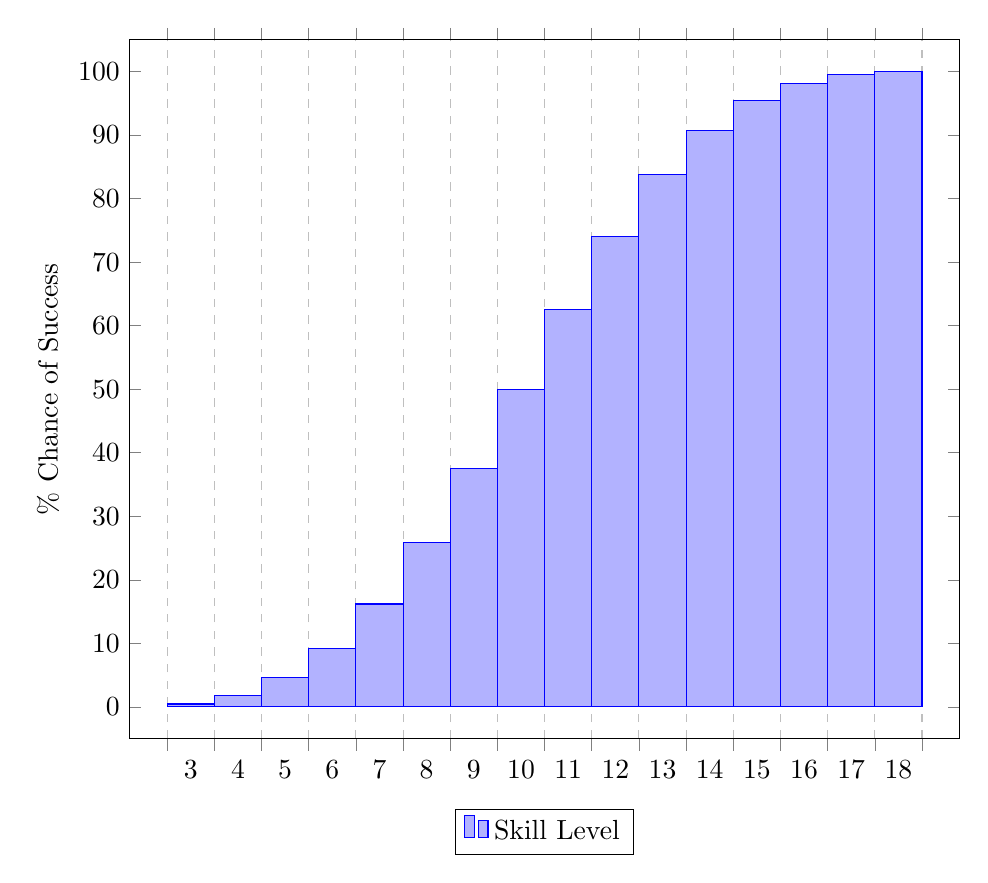
\begin{tikzpicture}
\begin{axis}[
	x tick label style={/pgf/number format/1000 sep=},
	ylabel=\% Chance of Success,
	enlargelimits=0.05,
	ytick = {0, 10, 20, 30, 40, 50, 60, 70, 80, 90, 100},
	legend style = {
	    at={(0.5,-0.1)},
	    grid style = dashed,
	    anchor=north,legend columns=-1
	},
	ybar interval = 1,
]
\addplot 
	coordinates {
	    (3,    0.46) 
	    (4,    1.85)
		(5,    4.63) 
		(6,    9.26) 
		(7,   16.20) 
		(8,   25.93) 
		(9,   37.50) 
		(10,  50.00) 
		(11,  62.50) 
		(12,  74.07)
		(13,  83.80)
		(14,  90.74)
		(15,  95.37)
		(16,  98.15)
		(17,  99.54)
		(18, 100.00)
		(19, 0)
	};
\legend{Skill Level}
\end{axis}
\end{tikzpicture}\\
The graph above shows the probability of succeeding a skill roll. If your character has an effective skill of 10, they have a 50\% chance of succeeding that roll. If they have a skill of 12, the chance of success goes up to 74\%.
\section{Critical Miss Table (Melee)}
\begin{center}
\begin{tabular}{r | l}
    \textbf{Roll} & \textbf{Result}\\\hline
    1 & Your weapon turns in your hand, and you hit with the flat side! \\
    2 & Your weapon breaks! \\
    3 & You lose your grip and the weapon flies out of your hand! \\
    4 & You lose your balance, and your turn! \\
    5 & You trip and fall! You have to get up again.\\
    6 & You hit yourself in the arm or leg! (50\% chance of hitting either)\\
\end{tabular}
\end{center}
\paragraph{Note}For \#3, the weapon flies 1d6 squares (50\% chance forward or backward). If it hits someone, it does half damage and lands there.

%% \section{Critical Miss Table (Ranged)}
%% \begin{center}
%% \begin{tabular}{r | l}
%%     \textbf{Roll} & \textbf{Result}\\\hline
%%     1 & Your weapon jams.\\
%%     2 &\\
%%     3 &\\
%%     4 &\\
%%     5 &\\
%%     6 &\\
%% \end{tabular}
%% \end{center}

\section{Weapons} \label{sec:weapons}
\subsection{Melee Weapons}
\begin{center}
\begin{tabular}{c|c|c|c|c|c}
    \textbf{Category} & \textbf{Name} & \textbf{Class} & \textbf{Damage} & \textbf{Damage Type} & \textbf{Range} \\\hline
    Unarmed  & Fists          & Light & d6-2 & Crushing & Close/1\\
             & Feet           & Light & d6-1 & Crushing & Close/1\\\hline
    Medieval & Short Sword    & Light & d6   & Slashing & Close/1\\
             & Long Sword     & Heavy & d6+2 & Slashing & 1 to 2 \\
             & Mace           & Heavy & d6+2 & Crushing & Close/1\\\hline
    Modern   & Baseball Bat   & Heavy & d6+1 & Crushing & Close/1\\
             & Aluminium Bat  & Light & d6+1 & Crushing & Close/1\\
             & Brass Knuckles & Light & d6-1 & Crushing & Close/1\\\hline
    Future   & Beam Sword     & Light & d6+3 & Slashing & Close/1
\end{tabular}
\end{center}

\subsection{Ranged Weapons}
\begin{center}
\begin{tabular}{c|c|c|c|c}
    \textbf{Category} & \textbf{Name} & \textbf{Damage} & \textbf{Damage Type} & \textbf{Accurate Range} \\\hline
    Primitive & Rock        & d6-1  & Crushing & $0.5 \times Shooting + Prof$  \\\hline
    Medieval  & Short Bow   & d6+1  & Piercing & $Shooting + Prof$ \\
              & Long Bow    & d6+2  & Piercing & $2 \times Shooting + Prof$ \\\hline
    Modern    & Pistol      & 2d6+2 & Crushing & 56m \\
              & Shotgun     & 5d6   & Crushing & 3m \\\hline
    Future    & Laser Gun   & 6d6   & Piercing & 66m \\
\end{tabular}
\end{center}
\paragraph{Note} These ranges are for when you want to shoot without a range penalty.
So despite the fact that a pistol can shoot around 1800m, it's incredibly hard to do so.

\section{Armour}
\begin{center}
\begin{tabular}{c|c|c|c}
\textbf{Category} & \textbf{Name}  & \textbf{PD} & \textbf{DR}\\\hline
         Medieval & Learther       & 1 & 1 \\
                  & Half Plate     & 2 & 2 \\
                  & Full Plate     & 4 & 3 \\
                  & Chain Mail     & 1 & 1 \\\hline
           Modern & Summer Clothes & 0 & 0 \\
                  & Winter Clothes & 0 & 1 \\
                  & Kevlar Vest    & 1 & 3 \\\hline
           Future & Polymer        & 4 & 3 \\
\end{tabular}
\end{center}

\chapter{Character Sheets}\label{app:character-sheets}
This Appendix contains some example character sheets as well as an empty one ready for printout.
\includepdf[pages = -]{graphics/character-sheet-example.pdf}
\includepdf[pages = -]{graphics/siren-character-sheet.pdf}
\end{document}

\chapter{Example Exploits}
Trying to come up with new exploits in the heat of the moment can be hard.
This appendix exists to alleviate this pain and get the proverbial juices flowing.

\section{Red Tape Recorder}
Persuasion is $Int + Int$ when dealing with government officials.
\documentclass[a4paper]{book}
\usepackage[utf8]{inputenc}
\usepackage[margin=3cm]{geometry} % For smaller margins
\usepackage{appendix} % For appendix support
\usepackage{tikz, pgfplots} % For the skill outcome graph
    \pgfplotsset{width = \textwidth, compat = newest}
\usepackage{graphicx} % For advanced picture insertion
\usepackage{pdfpages} % For inserting PDFs
\usepackage{multicol} % For supporting multi-columnar tables
\usepackage{tcolorbox} % For coloured info boxes
    \tcbuselibrary{skins}
    \tcbset{colback=brown!10, fonttitle=\scshape}
\usepackage{textcomp} % For the interrobang
\usepackage[sc,sf,bf]{titlesec} % for custom titles
\usepackage{sectsty} % for section styles
\usepackage{fancyhdr} % for "fancy" headers
\usepackage[notmath]{sansmathfonts} % for a sans-serif small-caps font
\usepackage{enumitem} % for finer control over enumerations
 
%%%%%%%%%%%%%%%%%%%%%%%%%%%%%%%%%
%% CHAPTERS & SECTION HEADINGS %%
%%%%%%%%%%%%%%%%%%%%%%%%%%%%%%%%%


% Simplifies chapter titles
% No longer says
% Chapter 2
% Game Creation
% but instead simply
% 2 Game Creation
\titleformat{\chapter}[hang]
{\sffamily\bfseries\scshape\Huge}
{\thechapter\quad}{0pt}{}{}

% Removes unnecessarily large margin above chapter title
\titlespacing*{\chapter}{0pt}{-\topskip}{40pt}

% Set the remaining titles to be sans serif and small caps
\allsectionsfont{\sffamily\scshape}

%%%%%%%%%%%%%%%%%
%% THUMB INDEX %%
%%%%%%%%%%%%%%%%%

\renewcommand{\chaptermark}[1]{\markboth{\textsc{\thechapter\ #1}}{}}

%%%%%%%%%%%%%%%%%%%%%%%
%% CUSTOM TEXT BOXES %%
%%%%%%%%%%%%%%%%%%%%%%%
\newtcolorbox{note}{
    enhanced, % enable advanced settings
    left = 10mm, % pushes text away from the left edge by 10mm
    sharp corners, % disables rounded corners
    rounded corners = southeast, % "round" the bottom right corner
    arc is angular, % make the "round" corner an angle
    arc = 3mm, % controls corner cut
    boxrule=0.6pt, % sets box line thickness
    underlay={%
        \path[fill=tcbcolback!80!black] ([yshift=3mm]interior.south east)--++(-0.4,-0.1)--++(0.1,-0.2); % triangle
        \path[draw=tcbcolframe,shorten <=-0.05mm,shorten >=-0.05mm] ([yshift=3mm]interior.south east)--++(-0.4,-0.1)--++(0.1,-0.2); % triangle edge
        \path[fill=gray!50!black,draw=none] (interior.south west) rectangle node[brown!10]{\Huge\bfseries \textinterrobang} ([xshift=8mm]interior.north west);
    },
    drop fuzzy shadow % adds drop shadow
}

\newtcolorbox{example}{
    enhanced,
    title = Example,
    before upper={\parindent15pt\noindent} % add paragraph indentation
}

\title{Siren - Simple RPG Engine $\beta1.0.1$}
\author{By Niko Lepka}
\date{\today}

\begin{document}

\maketitle

\chapter*{Preface}
\section*{What is Siren?}
Siren, the \textbf{Si}mple \textbf{R}PG \textbf{En}gine, is an RPG system that aims at being simple and easy to learn without also compromising on the expressiveness of the system.

An RPG engine, much like a video game engine, is a framework on which you can build your own system. If any of the rules in this seem like they don't \textit{quite} fit what you need, you're free to change them for your campaign

\section*{What are RPGs?}
Role Playing Games, or RPGs for short, are games in which you take the role of some character and act in their stead.
You may know this from video games, where you play some adventurer in a medieval land full of magic and dragons; or where you play a person that's trying to survive in a nuclear wasteland, fighting mutants and warring factions.
But RPGs date back before that.

Traditional RPGs, also known as \textit{Tabletop RPGs} or \textit{Pen and Paper RPGs} date back to the early 1970s.
It's a social game played with a group of friends around a table, mutually telling a common story of great adventure, mysticism, space warfare or whatever they can come up with.

\section*{Who is this for?}
Some role-playing systems have hundreds of books and rules, so many so that it's hard to remember them all, and valuable playtime is spent looking up rules. 
While other systems have so few and vague, that a lot of playtime is spent arguing about which rules apply to a given situation.

Siren is made for those players who wish to have a small yet precise set of rules that can be used in every type of story, whether it's a grand space opera, or high fantasy, Siren's got you covered.

\section*{Conventions}
This book uses standard RPG dice notation, which looks like this: $AdX\pm L$, where $A$ is the number of dice, $X$ is the number of faces on the die, and $L$ is the value added or subtracted after the roll, so $3d6+8$ means roll three six-sided dice, and add 8 to the result.
\paragraph{Note} Notes are displayed like this, and often convey important information to the player or GM regarding a certain mechanic.
\paragraph{Example} Examples are displayed like this, and show a situation in which something is used.

\newpage
\section*{Special Thanks}
Special thanks to the lovely individuals who've helped out with the project:
\begin{center}
    \begin{tabular}{cccc}
        Aleksander Øglænd & Christian J. Martinsen & Marco L.L. Olsen & Morten M. Rasmussen \\
        Patrick A. & Thomas G. McCollin \\
    \end{tabular}
\end{center}

\section*{Licence}
This work is licensed under the Creative Commons Attribution-ShareAlike 4.0 International License.
To view a copy of this license, visit http://creativecommons.org/licenses/by-sa/4.0/ or send a letter to Creative Commons, PO Box 1866, Mountain View, CA 94042, USA.

\tableofcontents

\chapter{Getting Started}
\section{What You Need}
\begin{enumerate}
    \item \textbf{Three to six players.} One of which will have to be the Game Master (GM).
    \item \textbf{Character sheets.} One per player. Additional paper is encouraged, but nor required.
    \item \textbf{GM sheet.} Special sheet for the Game Master.
    \item \textbf{Dice!} At least 3d6 per player, more is not necessarily required, but encouraged.
\end{enumerate}

\subsection{What's a Game Master?}
The Game Master is the special player in a game that directs the flow of the adventure.
The GM is responsible for narrating, setting up obstacles, and role-playing the Non-Player Characters (NPCs) that the players have to face throughout their adventures.

As a GM, the world is at your discretion. 
You roll the dice for everyone that isn't controlled by the players, you set the tone and mood of the environment, and you create the scenarios that will shape the decisions of the players.
You also get to set the difficulty of the obstacles at hand.

\subsection{The Role of the Player}
The player's role is to play their character, and face the trials imposed by the GM.
As a player, you control one of the protagonists in the story that the GM is telling, you make their choices and roll their dice to see how well they perform certain tasks.

\section{Character Sheet}

\section{Performing Actions}
Actions are what usually drives the plot in an RPG, whether it's talking to an NPC or performing great heroic feats, it's all actions.

Some actions have a chance of failure, and thus require you to roll your dice (typically 3d6) to see if you succeed or not. 
These are performed as \textit{Skill Rolls} and are covered more in depth in chapter \ref{chap:skills}. 
The success or failure of this roll decides the fate of your character.

Other actions succeed automatically, and do not require a skill roll, unless there's a very good reason that there should be.
Imagine having to roll your dice every time you wanted to talk to an NPC or walk down the street. 
Unless your character has crippling social anxiety or completely lacks a balance, it's assumed that these sorts of things are automatically successful.
\chapter{Game Creation}
\section{Telling a Story Together}
First and foremost, the point of playing an RPG is telling a story together, how you manage to go about doing so is completely up to you.
Creating a good story for your players to interact with can be a bit difficult at times, but it is absolutely doable.
Let your imagination run wild and see what you can come up with!
Generally speaking you need a few things:
\begin{itemize}
    \item A setting
    \item A scale
    \item A plot-line
    \item NPCs
\end{itemize}

\section{Setting}
The setting is one of the most important aspects of your game.
It determines everything from whether or not magic exists, to things like alien races, or level of technology.

Do you want to make 1940's style Noir story set in the distant future in a city that spans an entire planet? Go for it!
The most important thing, is that you---as the GM---can keep track of the setting, and keep it somewhat consistent.
Consistency is important so that things don't feel out of place. 
Don't be afraid to break consistency if you want to surprise or weird your players out.
It's your game world, make it however you want it.

\section{Scale}
When creating a game, it's also important to keep the scale of it all in mind.
Do you want a giant flourishing world filled to the brim with characters and opportunities on every corner? 
Or do you instead want something small and personal that can be wrapped up in a few sessions, but leaves a deep and profound impact on the players?
It's all up to you.
Just remember not to bite over more than you can chew.
It's easy to create this massive world and get lost in it.

\section{Plot}
What is a story without issues to resolve? Like any good movie or video-game, the story needs a plot-line.
Is a big evil corporation trying to take over the world?
Is a secret society conspiring against the general population?
Maybe a hoard of dragons are stealing all the magic in the world for themselves in preparation for an upcoming war.

It's up to you, make it good.

\section{Non-Player Characters}
What is a world if there aren't anyone in it?
Just like the players need characters, so does the game world.
It's important to remember not only to make major plot-related NPCs, like an spy in the organisation you're trying to infiltrate, or the big bad guy that is foiling your plans at every step.
But minor NPCs like the slew of goons you want your players to fight, or that one one-off clerk at the shop that the players want to interact with.

NPCs generally come in those two flavours: Major and Minor.
Major NPCs are best created with a full character sheet, like the players, but minor NPCs can make by with just the most important stats written down.
\chapter{Character Creation}\label{chap:char-creat}
\section{Introduction}
Character creation is perhaps one of the most important aspects of an RPG.
How you design your character impacts how the game is going to be played.
This chapter is meant as a guide to help you through creating your character in Siren. 
Appendix~\ref{app:character-sheets} has a blank character sheet for you to copy.

\begin{note}
    All fractions are rounded down by default unless explicitly stated otherwise.
\end{note}

\section{Use Your Imagination}
Make your character yours.
Think of a back-story for them, give them a reason to exist in the world you're playing in.
If you are unsure about what works in the setting, ask your GM for help; after all, they're the one curating the game.
Work with the GM and the other players to create a character that best works for your game.

\begin{note} 
    The following is meant as a loose guide.
    If the GM decides, any and all of the rules below can be changed to suit your particular game.
\end{note}

\section{The Character Sheet}
The character sheet comes in three pages.
\paragraph{Page 1} The general stats page, which contains your traits, skills, and exploits.
\paragraph{Page 2} The weapons, spells, and armour page, which keeps track of your weapons, spells, armour, and shields.
\paragraph{Page 3} The character and possessions page, which keep track of your character notes (back-story, etc.), money, and loot.
Example character sheets have been included in Appendix~\ref{app:character-sheets}.

\begin{note} 
    In case you can't fit on everything on the character sheet, feel free to use the reverse side of the paper!
\end{note}

\section{Building a Character}
\subsection{Experience Points (XP)}
To help you out, you'll get \textbf{35 XP} to start out (The GM may decide to give more or less XP depending on setting or circumstance).
These can be used to purchase skill specialisations and upgrade your traits if you so desire at the beginning of the game.
Check Chapter~\ref{chap:char-prog} for more information about how XP works.

\subsection{Traits}
During character creation, each trait level costs 1 XP and cannot exceed a trait level of 10.

The derived traits are calculated like this:
\begin{center}
\begin{tabular} {r | l} 
\textbf{HP:} & $Con \times 2$ \\
\textbf{FP:} & $Con + Str$ \\
\textbf{MP:} & $Int \times Wis$ \\
\textbf{Speed:} & $Athletics / 2$\\
\textbf{Parry:} & $Fighting / 2 + \mathit{DfM}$\\
\textbf{Dodge:} & $Speed + \mathit{DfM}$ \\
\end{tabular}
\end{center}
See Section~\ref{sec:skills-in-depth} for Athletics, and Section~\ref{sec:defence} for an explanation on \textit{Parry}, \textit{Dodge}, and \textit{DfM}.

\begin{note} 
    The \textit{Parry} box on the character sheet is split in two, this is due to the fact that there are \textit{two} parry traits: one for \textit{Fighting (Heavy)} and one for \textit{Fighting (Light)}.
    It is up to you which half to use for which, as long as you can remember it.
\end{note}

\begin{example}
A character with the traits set up like this:

\begin{center}
    \begin{tabular}{ccccccc}
        \textbf{Agi} & \textbf{Cha} & \textbf{Con} & \textbf{Dex} & \textbf{Int} & \textbf{Str} & \textbf{Wis} \\\hline
        6 & 4 & 4 & 6 & 5 & 4 & 3\\ 
    \end{tabular}
\end{center}
Would cost 32 XP to build.
Note that a value of 5 is considered \textit{average}.

See Appendix~\ref{app:character-sheets} for an example character with these exact traits.
\end{example}

\subsection{Skills}
Calculate your character's skills based on their traits as shown in the skill listing on your character sheet.
Think about what your character is particularly good at, these skills can be what your character specialises in.
See Chapter~\ref{chap:skills} for more information about Skills in general.

\subsection{Exploits}
Exploits are entirely player-defined, and are a way of personalising your character to fit your play-style.
Exploits can range from simply providing bonuses, to providing exceptions to the existing rules.
You can read more about exploits in Chapter~\ref{chap:exploits}.

\subsection{Weapons}
The weapons section of the character sheet lists all the relevant attributes of a given weapon.
The section is divided into five columns: \textit{name}, \textit{specialisation}, \textit{damage \& type}, \textit{range}, and \textit{parry}.

\paragraph{Name} The given name of the weapon, this could be something as simple as ``Long Sword'' ``Glock~22'' to something as personal as ``Widow-Maker'' or ``Demon Slayer''.

\paragraph{Specialisation} The name of the given specialisation the weapon falls under.
The idea is that, if you're able to use one long sword, you're able to use all of them, doesn't matter if one has a fancier handle than the other. 
The specialisation is also what you upgrade if you want to be better at using the weapon.
You can think of this as the \textit{weapon class}.

\paragraph{Damage \& Type} The dice you roll and the type of damage it deals.
Examples include $2d6\ \mathit{Piercing}$ and $1d6+3\ \mathit{Crushing}$.

\paragraph{Range} The range of the weapon in meters.
The range of a weapon is most useful when playing with a game mat (see Chapter~\ref{chap:combat}), where the width of each square corresponds to $1m$.

\paragraph{Parry} The individual weapon's parry score, which differs from the score in the box on the front of the character sheet.
It is included here for quick reference.

This is the \textit{Parry} score from the first page, plus the weapon's specialisation.

\subsection{Shields \& Armour}
The shields and armour sections list the relevant attributes of your characters' defensive equipment.
Where they differ, is in the fact that shields can be used offensively as well as defensively.
Shields share all columns as weapons except range, as all shields are considered close-range weapons.
Therefore, refer to the relevant columns in the weapons section above.

The defensive stats for shields and armour are divided into \textit{DfM} and \textit{Damage Resistance}.
Refer to Section~\ref{sec:defence} for more info.

\paragraph{DfM} Short for \textbf{D}e\textbf{f}ence \textbf{M}odifier.
It is a type of passive bonus applied to your \textit{Dodge} and \textit{Parry}, which makes it more likely for you to not get hurt during combat.

\paragraph{Damage Resistance} Provides damage reduction in the case you \textit{do} get hit.
Damage Resistance makes attacks hurt less, thus increasing your survivability during combat.

\subsection{Spells}
The spell section lists the spells your character knows and is able to use.
The section is divided into \textit{name}, \textit{cost}, and \textit{description}.
Check Chapter~\ref{chap:magic} for more information about magic in general.

\paragraph{Name} The name of the spell.
Unlike weapons, spells don't fall into general categories in quite the same way, so specialisations need to be handled on a per-spell basis.
It's important to note, that just because your character doesn't specialise in a given spell, it doesn't also mean they can't use it.
It is ultimately up to the GM to decide whether a spell can be learned or not.

\paragraph{Cost} The cost of the spell in $MP$.
Some spells consume mana-points, which limit the number of times a spell can be used.
See Section~\ref{sec:mana} for more details.

\paragraph{Range} The range of the spell.
Depending on the setting, the range of any given spell can vary widely from point-blank to several kilometres.

\paragraph{Description} Describes the effects of the spell in question.
Things like how it behaves and---if applicable---how much damage it deals.

\subsection{Equipment}
The equipment section lists all the stuff you're carrying.
This is everything from armour and clothes, to loot, to weapons.

\subsection{Money}
Each box in the money section is for the type of the currency carried, and the lines next to the boxes are meant for the amount of said currency.
So if you're playing an international spy, the boxes could hold \textit{USD}, \textit{GBP}, \textit{EUR}.
And if you're playing in a fantasy setting, they could hold \textit{Gold}, \textit{Silver}, \textit{Bronze}.

\begin{example} 
Here's an example of how the money table on the character sheet could be filled in a medieval fantasy setting:
\begin{center}
    \begin{tabular}{|r|l@{\hspace{1cm}}}\cline{1-1}
        Platinum & 0\\\hline
        Gold & 12\\\hline
        Silver & 144\\\hline
        Copper & 59\\\hline
               & \\\hline
    \end{tabular}
\end{center}
\end{example}
\section{Adding or Changing Traits}
Your setting may not be satisfied with just the seven basic traits included in the core rules.
It could be that you feel it would be better with an eighth trait like \textit{Faith} or \textit{Psionics} or something else entirely.
Maybe you instead prefer combining some of the traits into broader categories, like combining \textit{Int} and \textit{Wis} into a joined \textit{Mental} trait.
It's all doable, should you want to do so.
Just keep in mind: it's easier to add traits than to remove or combine them, since the latter will inevitably require you to rewrite many of the \textit{Skills} to fit the new listing.
\chapter{Skills} \label{chap:skills}
\section{Introduction}
Skills are the primary workhorse in the game. 
Whenever there's any situation that requires action, a player rolls against their skill plus/minus modifier. 
There are 18 different skills, as seen in figure \ref{fig:skills}. 
These skills reflect the different types of actions a player can perform during play.


\section{Skill Rolls}
The player rolls three six-sided dice (3d6) against their skill of choice, if the outcome is $\leq$ the skill level, it's a success, if not, it's a fail.
Rolling a 3, is an automatic success (regardless of level), and rolling an 18 is an automatic fail (also regardless of level).

\paragraph{Example} Say Alice wants to persuade a guard to do something stupid. Her \textit{Persuasion} skill is at 13. 
She rolls 3d6, and rolls a 1, a 5, and a 3, which is 9 in total. This means she successfully persuades the guard.

\begin{figure}
\centering
\begin{tabular}{r | c | c | l}
\textbf{Category} & \textbf{Skill}   & \textbf{Traits} & \textbf{Description} \\\hline
    Mental    & Academics        & $Int+Int$ & Use vast knowledge of a certain field.        \\
              & Investigation    & $Int+Wis$ & Searching for things and information.         \\
              & Magic            & $Int+Wis$ & Perform fantastical feats.                    \\
              & Perception       & $Int+Wis$ & The passive ability to spot things.           \\
              & Survival         & $Con+Int$ & Surviving in certain environments.            \\
              & Thievery         & $Dex+Int$ & Performing certain larcenous activities.      \\\hline
    Physical  & Athletics        & $Agi+Con$ & Perform a certain task that requires stamina. \\
              & Fighting (Heavy) & $Agi+Str$ & The ability to fight with heavy weapons.      \\
              & Fighting (Light) & $Agi+Dex$ & The ability to fight with light weapons.      \\
              & Physique         & $Con+Str$ & Any action that requires strength.            \\
              & Stealth          & $Agi+Wis$ & Sneaking around and acting unseen.            \\\hline
    Social    & Contacts         & $Cha+Int$ & Make and use connections with people.         \\
              & Insight          & $Cha+Wis$ & Sensing and social cues and motivation        \\
              & Nursing          & $Cha+Wis$ & Taking care of people                         \\
              & Persuasion       & $Cha+Wis$ & Manipulating people.                          \\\hline
    Technical & Crafting         & $Dex+Int$ & Making things with your hands.                \\
              & Shooting         & $Dex+Wis$ & Shooting or throwing objects.                 \\
              & Vehicle (Air)    & $Dex+Wis$ & Operating motorised air vehicles.             \\
              & Vehicle (Land)   & $Dex+Wis$ & Operating motorised land vehicles.            \\
              & Vehicle (Sea)    & $Dex+Wis$ & Operating motorised sea vehicles.             \\
\end{tabular}
\caption{Skill Listing}
\label{fig:skills}
\end{figure}
\newpage
\section{Proficiency \& Specialisation}
Your character can specialise in any number of different skills.
Specialising grants the skill a \textit{Proficiency Bonus} of $+3$ to that particular specialisation.

\paragraph{Note} Just because your character hasn't specialised in anything, does not mean they cannot perform it, it just means they don't get the proficiency bonus.

\paragraph{Example} Joyce is an Olympic runner, and has a \textit{Constitution} of 5, and an \textit{Agility} of 5; this gives her an \textit{Athletics} score of 10. 
As a runner, she specialises in running, which grants her a $+3$ bonus to her \textit{Athletics} roll whenever she needs to perform a running task.
She rolls 11, but because her effective \textit{Athletics} score is 13 due to the bonus, she succeeds.

\newpage
\section{Skills in Depth}
\subsection{Mental Skills}
\subsubsection{Academics (Int + Int)}
The Academics skill, called \textit{Knowledge}, or \textit{Lore} in other games, is the skill of knowing things factually. 
This can be things your character has read, or something they've researched.
If your character needs to identify ancient writing, source herbs, design circuits, or have a meaningful discussion with an expert, this is the go-to skill.

\paragraph{Specialisations:}
\begin{center}
    \begin{tabular}{c|c|c|c}
        Maths & Physics & Chemistry & Theology \\
        Medicine & Literature & Linguistics & History \\
        Anthropology & Computer Science & Magic & Botany \\
        Geology & Astronomy & Quantum Physics & Computer Security \\
    \end{tabular}
\end{center}

\subsubsection{Investigation (Int + Wis)}
Investigation is the skill of actively searching for things and gathering information.
Whether your character is hunting for clues or digging through books, investigation is the skill to use.

\subsection{Magic (Int + Wis)}
Magic is the skill of performing fantastical things with power channeled through the body.
Whether it's chi energy, spiritual power, nanobots, genetic modification, or the essence of the universe that powers your abilities, it all falls under \textit{Magic}.

\paragraph{Specialisations:}
\begin{center}
  \begin{tabular}{c|c|c|c}
    Life & Construction & Destruction & Utility \\
    Earth & Water & Air & Fire \\
    Arcane & Black/Dark & White/Light & Temporal \\
    Divine & Diabolic
  \end{tabular}
\end{center}
Magic is covered much more in depth in chapter \ref{chap:magic}.

\subsubsection{Perception (Int + Wis)}
Perception, called things like \textit{Notice} or \textit{Awareness} in otehr games, is the skill of using your senses to \textit{passively} notice what's going on around you.

\subsubsection{Survival (Con + Int)}
Survival is the skill of surviving; particularly in inhospitable environments.

\paragraph{Specialisations:}
\begin{center}
    \begin{tabular}{c|c|c|c}
        Desert & Tundra & Jungle & Island \\
        Prairie & Urban & Off-World & Space \\
        Under Water & Underground & Mountain & Arctic \\
    \end{tabular}
\end{center}

\subsubsection{Thievery (Dex + Int)}
Thievery is a catch-all term for general larcenous and/or criminal skills that (generally) involve thought and finesse.
These skills are regarded as such regardless of their actual use.

\paragraph{Specialisations:}
\begin{center}
    \begin{tabular}{c|c|c}
        Pick-Pocket & Lock-Pick & Sleight of Hand \\
        Alarm Deactivation & Hacking & Evidence Tampering \\
    \end{tabular}
\end{center}

\subsection{Physical Skills}
\subsubsection{Athletics (Agi + Con)}
Athletics, sometimes called \textit{Endurance} in other games, is a skill that has your character perform physically challenging things, often involving swiftness or stamina.
Tasks such as running, climbing, or swimming fall under here.

\paragraph{Specialisations:}
\begin{center}
    \begin{tabular}{c|c|c|c}
        Running & Climbing & Swimming & Jumping \\
        Acrobatics & Biking & Diving & Sailing \\
    \end{tabular}
\end{center}

\paragraph{Note} Sailing here refers to sailing a non-motorised sail or row boat. For motorised sailing, see the skill \textit{Driving}.

\subsubsection{Fighting (Heavy) (Agi + Str)}
This is the skill of melee fighting with heavy weaponry. Weapons such as clubs, mallets, war-hammers, axes, etc. fall under this skill.

\paragraph{Specialisations:}
\begin{center}
    \begin{tabular}{c|c|c|c}
        Mace & Club & Mallet & War Hammer \\
        Claymore & Baseball Bat & Pipe & Pipe Wrench \\
        Battle Axe & Two-by-Four & Odachi & Talwar \\
    \end{tabular}
\end{center}

\subsubsection{Fighting (Light) (Agi + Dex)}
This is the skill of melee fighting without weapons or wit light weaponry. 
Weapons such as rapiers, short swords, lances, and knives fall under here.

\paragraph{Specialisations:}
\begin{center}
    \begin{tabular}{c|c|c|c}
        Rapier & Short Sword & Katana & Beam Sword \\
        Knife & Ice Pick & Baton & Brass Knuckles \\
        Fist (punching) & Foot (kicking) & Rolling Pin & Letter Opener \\
    \end{tabular}
\end{center}

\subsubsection{Physique (Con + Str)}
Physique, the raw strength counterpart to Athletics. 
This skill involves everything that requires strength.
Lifting, pulling, or pushing heavy objects are things that fall under here.

\subsubsection{Stealth (Agi + Wis)}
Stealth is the act of moving around unnoticed.
Tasks such as blending in, sneaking, and infiltrating all fall under here.

\subsection{Social Skills}
\subsubsection{Contacts (Cha + Int)}
Contacts is the skill of creating, maintaining, and making use of contacts.
So if your character needs to call a friend for help, or establishing a new connection with someone for use later, this is the skill for you.

\subsubsection{Insight (Cha + Wis)}
Insight, called \textit{Sense Motive} or \textit{Empathy} in other games, is the dual/opposite of \textit{Persuasion}. 
This skill is all about reading people and their intentions, and trying to figure out what they're up to.
So if you're suspecting a salesman is trying to scam you, or if you're trying to figure out if an unstable inmate is about to have a wild mood swing, this is the go-to skill.

\subsection{Nursing (Cha + Wis)}
The Nursing skill is all about taking care of animals and people and making them feel good.
A good nurse can have a positive effect on someone's mental and physical health, and in fact can help speed up their natural healing.

\subsubsection{Persuasion (Cha + Wis)}
Persuasion is the skill for manipulating people for good or bad.
Whether you need to lure a guard away from his post, trick the evil sorcerer to reveal his secret plan, or strike a favourable deal with the mob boss, or maybe you just want to sit around in a pub cracking jokes, lightening the mood of the people around; this is the skill you want to use.

\paragraph{Specialisations:}
\begin{center}
    \begin{tabular}{c|c|c|c}
        Bargaining & Charming & Convincing & Inciting \\
        Seducing & Taunting & Provoking & Distracting \\
        Rapport & Deception & Bluffing & Intimidation
    \end{tabular}
\end{center}

\subsection{Technical Skills}
\subsubsection{Crafting (Dex + Int)}
The skill of making things, any hobby or task that involves producing something tangible with your hands belongs here.

\paragraph{Specialisations:}
\begin{center}
    \begin{tabular}{c|c|c|c}
        Paper Crafts & Origami & Carpentry & Woodworking \\
        Masonry & Smithing & Machining & Electronics \\
        Gadgeteering & Knitting & Casting & Sculpting \\
    \end{tabular}
\end{center}

\subsubsection{Vehicle, Air (Dex + Wis)}
The act of operating an airborne vehicle.

\paragraph{Specialisations:}
\begin{center}
    \begin{tabular}{c|c|c|c}
        Plane & Jet & Helicopter & Hot Air Balloon \\
        Commercial Liner & Zeppelin & Flying Car \\
    \end{tabular}
\end{center}

\subsubsection{Vehicle, Land (Dex + Wis)}
The act of operating land vehicles.

\paragraph{Specialisations:}
\begin{center}
    \begin{tabular}{c|c|c|c}
        Car & Truck & Tractor & Tank \\
        Train & Moped & Motorcycle & Hovercraft
    \end{tabular}
\end{center}

\subsubsection{Vehicle, Sea (Dex + Wis)}
The act of operating water based vehicles.
Note that sailing sail/row boats are Olympic disciplines, and thus fall under \textit{Athletics}.

\paragraph{Specialisations:}
\begin{center}
    \begin{tabular}{c|c|c|c}
        Jet-Ski & Motor Boat & Yacht & Cruise Liner \\
        Submarine & Hovercraft & 
    \end{tabular}
\end{center}

\subsubsection{Shooting (Dex+Wis)}
Shooting is the skill of launching projectiles, whether it be by throwing, or launching them from a device.

\paragraph{Specialisations:}
\begin{center}
    \begin{tabular}{c|c|c|c}
        Throwing & Slingshot & Bow & Crossbow \\
        Pistol & Revolver & SMG & Rifle \\
        Assault Rifle & Cannon & Ballista & Trebuchet \\
        Mortar & Tank Turret & Helicopter Turret & Blowpipe
    \end{tabular}
\end{center}

\newpage
\section{Contest of Skills}\label{sec:contest}
Situations arise, when your character needs to test their skills and prove their worth, this is done via a \textit{Contest of Skills}.
These contests come in three different variants: \textit{Passive}, \textit{Active}, and \textit{Tournament}.

\subsection{Passive Contest}
A passive contest arises when the character needs to overcome some passive obstacle. This could be things like walking a tightrope, picking a lock, leaping over a gap, etc.
The GM silently decides the level of difficulty by announcing a skill +/- a modifier that needs to be rolled.

\paragraph{Example} Astrid is running from her pursuers across the rooftops of ancient Rome, she needs to clear a particularly wide gap between the buildings. Astrid says \textit{``I'm jumping the gap''}, to which the GM replies \textit{``Roll Athletics -2''}. Astrid's Athletics skill is at 11, at -2, she must roll 9 or less to succeed. She rolls an 8 and gracefully leaps between the buildings.

\subsection{Active Contest}
An active contest is when the character is up against someone or something that actively works against them. Be it trying to pick-pocket a guard, an intense sword-fight, or playing chess against an opponent; all of this providing an \textit{active} resistance.

In an active contest, both parties roll against their most applicable skill, the outcome is judged as follows:

\begin{center}
    \begin{tabular}{c|c|c}
    \textbf{Character A} & \textbf{Character B} & \textbf{Winner}\\\hline
    Fail & Fail & The one failing by least \\
    Fail & Success & Character B \\
    Success & Fail & Character A \\
    Success & Success & The one succeeding by most
    \end{tabular}
\end{center}
If no one fails or succeeds more than the opponent, re-roll.

\paragraph{Example} Tom wants to sneak past a guard, Tom's \textit{Stealth} is at 9, he rolls 11, failing by 2 degrees. 
The guard's \textit{Perception} is at 10, but rolls 13, failing by 3 degrees. 
Tom failed less than the guard, thus successfully sneaking past the guard.

\subsection{Tournaments}
Tournaments are \textit{longer} contests of skills.
Tournaments are divided into rounds, whoever wins the most rounds wins the tournament.
Each individual round is a regular \textit{active contest}.

\chapter{Example Exploits}
Trying to come up with new exploits in the heat of the moment can be hard.
This appendix exists to alleviate this pain and get the proverbial juices flowing.

\section{Red Tape Recorder}
Persuasion is $Int + Int$ when dealing with government officials.
\chapter{Magic} \label{chap:magic}
\section{Introduction}
Some campaigns are set in a fantastical world, full of weirdness, improbable events, and of course: magic.
It is said that any technology that is sufficiently advanced, is completely indistinguishable from magic.
For this reason, we define the term \textit{Magic} to be a bit looser than traditionally.
So, whether we're talking beam sword wielding space wizards, battle mages, or even mutated people that gain power from sea slug juices;
if it seems to give super natural powers, it all just falls under this category.

\paragraph{Note} Spells are anything that is channelled through your body, regardless of how.
Whether the powers were given to you, or you were born with them, doesn't matter.

\section{Spells}
In order to cast a spell, it needs to be known to the character using it.
That is to say, it must be available on the character sheet in some capacity---either in the spell section or perhaps even as an item, depending on how the given setting deals with this.
For all intents and purposes, spells are treated like normal skill checks.

In other words, casting a spell requires two things: A skill roll, and---if the setting calls for it---enough mana.
Like all other skills, spells have four different outcomes, but being magic in nature, they act a bit differently from regular skills:
\begin{itemize}
  \item \textbf{Critical Success.} The spell is performed at double strength, at no extra cost.
  \item \textbf{Success.} The spell succeeds as intended.
  \item \textbf{Fail.} The spell is not performed, but MP is still lost.
  \item \textbf{Critical Fail.} The spell backfires at the GM's or the setting's discretion.
\\This could be the spell having negative unforeseen consequences, and/or the loss of MP.
\end{itemize}

\paragraph{Note} It's up to the GM or the setting to determine the difficulty of a spell.
The difficulty would be set as a $\pm$ skill modifier on the given spell.

\subsection{Affecting the Spells}
Spells come in many different forms: utility, healing, hurting, elemental, bionic etc.
Every spell has an associated mana cost, which consumes a bit of your total mana on each use (see Section~\ref{sec:mana}).

It's up to the players and the GM to decide the kinds of spells that exist within the game, and whether they're too game breaking or not.
Spells can be cast in four different ways:
\begin{enumerate}
  \item On yourself.
  \item Around you.
  \item Away from you.
  \item On someone else.
\end{enumerate}
Depending on the exact nature of that spell, these four casting methods can have vastly different effects, or even be unavailable altogether.

\paragraph{Example} Casting a shield spell on yourself grants you protection.
Casting it around you creates a bubble around you that can shield yourself and your friends.
While casting it away from you can create a wall to shield something/someone further away.

\section{Mana (MP)}\label{sec:mana}
Every character has a mana pool $Int \times Wis$ in size, which represents the amount of magical potential your character can tap into without straining themselves.
In other words, if your character has 5 Int, and 6 Wis, they have 30 Mana Points (MP).
Every spell has an associated mana cost, and using it drains the mana pool accordingly.

\subsection{Running Out of Mana}
When you run out of mana, your can still cast spells!
However, instead of draining mana, your character will instead accumulate 2 Fatigue Points (FP) for every point of mana attempted to use.

\subsection{Regaining Mana}
Mana is regained automatically over time.
About one point every 30 in-game minutes while not at rest,
a point every 10 minutes while relaxing,
and a full restoration after a good night's sleep.

If the setting allows it, mana potions can also help restore some of the spent mana.

\section{Acquiring New Spells}
You can cast any spell your character would logically be acquainted with within the boundries of the setting.
It is, however, up to the GM to decide the number of spells you are allowed to start out with.
Spell familiarity is determined through the skill proficiency system, see Chapter~\ref{chap:skills} for more info.

By default however, the GM decides the XP cost of any given spell, or whether or not characters have \textit{spell slots} that limit the number of spells held. 
The actual intricacies of how a spell is learned is also up to the GM.

\paragraph{Note} In a setting, where it has been decided by the GM that a scroll needs to be found and read in order to learn a spell.
It is possible for the skill check to learn and/or cast the spell is too difficult for the character's current skill level.
This means, XP need to be dedicated to the given spell in order to properly learn it.
\chapter{Combat}
\section{Introduction to Combat}
Combat is a staple of most RPGs. 
It's intense, often exhilarating, and it gives the players a chance to strategise. Combat is essentially a series of \textit{Contests of Skill} (see section \ref{sec:contest}), but due to the nature of combat are naturally a bit more involved.
\subsection{Turns}
Combat is split into a number of turns, each turn represents about 6 seconds of in-game time, meaning 10 turns make up an in-game minute.

\paragraph{Note} One turn is the time it takes for every character to have had a go, not the time for each individual character.
\subsection{Turn Order}
To determine turn order, each player rolls $1d6+Athletics$. The turn-order is then ordered highest to lowest. Highest result goes first, lowest goes last. Any ties require a re-roll.

\paragraph{Example} Alice, Bob, and Clarice all roll for turn order. They have an athletics score of 9, 9, and 10 respectively. Alice rolls a 5, Bob rolls 3, and Clarice rolls a 6. Clarice goes first with 16, Alice is next with 14, and Bob is last with a score of 12.

\subsection{Simple Vs. Advanced Combat}
Siren supports two different styles of combat: \textit{simple}, and \textit{advanced}.

Simple combat is the most straightforward, and involves nothing more than your character sheets and your imagination. A drawn map to help visualise the space is nice, but not required.

Advanced combat, on the other hand, uses a battle mat divided into squares. This mat is used to communicate the exact position of characters and NPCs, and helps visualise movement and trajectories on the battlefield.

\subsection{Active Defence}
Active defence differs from the \textit{Defend} action in that it occurs on the attacker's turn.
There are two things a character can do when actively defending:
\begin{enumerate}
    \item \textbf{Dodge.} Roll against your \textit{Move} trait.
    \item \textbf{Parry.} Roll against half of your weapon skill, rounded down.
\end{enumerate}
You get an additional $+2$ to your roll if you also choose to move out of the way of the attack.

\newpage
\section{Simple Combat}

\subsection{Attack (Melee)}
\begin{enumerate}
    \item Roll against the appropriate weapon skill.
    \item If you succeed, the opponent gets to roll active defence.
    \item If the defence fails, roll for damage for the appropriate weapon.
\end{enumerate}

\subsection{Attack (Ranged)}
\begin{enumerate}
    \item Calculate effective skill level.
        \begin{enumerate}
            \item Target is \textbf{close}: Use base-skill.
            \item Target is at \textbf{medium} range: $Skill-3$.
            \item Target is \textbf{far}: $Skill-6$.
            \item Target is \textbf{very far}: $Skill-9$.
        \end{enumerate}
    \item Roll to attack, using the modified skill.
    \item If you succeed, target opponent may roll to dodge.
    \item If the dodge fails, roll for damage.
\end{enumerate}

\subsection{Defend}
Spend your turn doing nothing but defending. 
You get an additional $+2$ to your active defences. 
You may not attack during this turn.

\subsection{Long Action}
Any non-combat task that takes more than one turn is a \textit{long action}.
Examples of long actions could be picking a lock, untying someone, calling for backup, or applying bandages.

\subsection{Prepare Action}
Prepare an action to be triggered at a specific moment.
This can be waiting to hit someone until they're about to draw their sword, waiting for someone to turn around before hitting them in the head, or waiting for your opponent to reload their weapon before casting a spell.

\newpage
\section{Advanced Combat}
Advanced combat is much like simple combat, except it uses a battle mat. Because of this, the different possible actions in a turn are affected by this addition.

\subsection{Movement}
Particularly, the characters rely on their movement points to move about the battle mat.
Movement is 8-directional (see figure \ref{fig:directions}), and moving in any direction costs 1 movement point.

\begin{figure}
    \centering
    \includegraphics{graphics/directions.png}
    \caption{The eight movement directions}
    \label{fig:directions}
\end{figure}

Your character can only move as far as their movement points allow, but you may choose to move a shorter distance if you so desire. Figure \ref{fig:movement} shows an example of a character moving 4 squares, which is worth 4 movement points.

\begin{figure}
    \centering
    \includegraphics{graphics/movement.png}
    \caption{Example of movement.}
    \label{fig:movement}
\end{figure}

\subsection{The Grid}
The battle mat is subdivided into a grid of squares. 
The in-game size of a square is $1m^2$, although the GM may scale it up or down as necessary.
The GM must alert the players of the scale if it differs from the standard $1m^2$.

\subsection{Actions}
\subsubsection{Long Action}

\subsubsection{Move \& Attack (Melee)}
\begin{enumerate}
    \item Move up to half your movement (rounded down) before or after attacking.
    \item Roll against the appropriate weapon skill.
    \item If you succeed, the opponent gets to roll active defence.
    \item If the defence fails, roll for damage for the appropriate weapon.
\end{enumerate}

\subsubsection{Move \& Attack (Ranged)}
\begin{enumerate}
    \item Move up to half your movement (rounded down) before or after attacking.
    \item Calculate effective skill level.
        \begin{enumerate}
            \item If target is within weapon's range, do nothing else.
            \item Subtract 3 points every time you exceed the range.
        \end{enumerate}
    \item Roll to attack, using the modified skill.
    \item If you succeed, the opponent may roll to dodge.
    \item If the dodge fails, roll for damage.
\end{enumerate}

\paragraph{Example} Will the Ranger is out hunting for his party. He spots a deer in the distance. His bow has a range of 100 metres, the deer is 300 metres away. This exceeds the bow's range twice ($2\times -3$ penalty). Will must roll $Longbow-6$ to succeed.

\subsubsection{Move \& Defend}
Move up to half your movement (rounded down) before defending. 
Spend the rest of your turn doing nothing else. 
You get an additional $+2$ to your active defences. 
You may not attack during this turn.

\subsubsection{Prepare Action}
Prepare an action to be triggered at a specific moment.
This can be waiting to hit someone until they step into the square in front of you, waiting for your opponent to reload their weapon before casting a spell, or waiting for a party member to stand in the square next to you before charging at the enemies.

\subsubsection{Relocate}
Move as far as your movement score allows and do nothing else.
Roll \textit{Athletics} to run, this doubles your range if you succeed.
If you fail you trip and fall prone.
If prone you may try to get up again on your next turn.
\chapter{Defence \& Damage Resistance}\label{chap:defence}
\section{Introduction}
Let's face it, taking damage isn't fun, but unfortunately, it's a natural and almost unavoidable consequence of combat.
Luckily, there are ways to avoid, or at least mitigate some of the damage taken.
For this, there are three different things that might help you out: damage resistance, and active and passive defence.

\section{Active Defence}
Active defence (AD), is performed by your character during combat.
This refers to actions like dodging, blocking, or parrying an attack.
More often than not, active defences have a very low chance of success, but also have a very high reward, as they make it possible to completely avoid all damage from an attack.

There are two things a character can do when actively defending:
\begin{enumerate}
    \item \textbf{Dodge.} Roll against your \textit{Speed} trait.
    \item \textbf{Parry.} Roll against half of your weapon skill, rounded down.
\end{enumerate}
You get an additional $+2$ to your roll if you also choose to move out of the way of the attack.

\section{Passive Defence}
Passive defence (PD), is defence gained from your armour.
Generally, thicker armour usually grants a bigger passive defence bonus.
The passive defence is added to your active defence score when performing a defence roll.

\paragraph{Example} Jean has been challenged by a rival clan's champion, who is charging at him, claymore raised high.
Jean's dodge is 6, his leather armour and buckler give him 1 PD each.
Added together, it gives him an effective defence of 8, which he then needs to roll against to evade the foe.
He rolls an 8! He slips right past his opponent, deflecting the claymore with his buckler.

\section{Damage Resistance}
Damage resistance (DR), is something that always applies, whether your character is aware of the attack or not.
Damage resistance is granted by certain armour, shields, and potions, and reduce some of the damage your character takes when hit.
Simply put: if your character has 2 points of damage resistance, then they take 2 points of damage fewer than they otherwise would.

\paragraph{Example} Cass the Paladin is in a fight to the death against the fearsome black knight.
She wears a steel breastplate, which grants a damage resistance of 3.
The black knight swings at her and she misses her dodge!
The black knight's sword damages for 6, but because of her armour's damage resistance, she only takes 3 damage!

\chapter{Character Progression}\label{chap:char-prog}
\section{Introduction}
Character progression is important in any RPG.
As your character progresses throughout the adventure, they're naturally going to acquire new abilities, and hone existing their skills.

\section{Experience Points}
To let your characters progress, the game uses \textit{Experience Points} (XP).
XP are used for three things:
\begin{enumerate}
\item Buy proficiency bonuses.
\item Buy trait upgrades.
\item Buy new exploits.
\end{enumerate}
The XP cost for each varies depending on what's being bought.

\section{Buying Proficiency Bonuses and Trait Upgrades}
The price of buying a proficiency bonus or trait upgrade is the same:
Each level costs itself in points.
Put differently: going from level 1 to 2 costs 2 points, and going from 7 to 8 costs 8 points.
Naturally, this means that if you want to buy three levels all at once, you have to pay the price of each successive level.

\paragraph{Example} Joyce wants to increase her warrior's \textit{Wisdom}, it's currently at level 2, and she wants to bring it up to level 5.
To make this happen, she needs to pay 12 XP, because she also needs to buy levels 3 and 4, making it $3 + 4 + 5 = 12$ XP.

\section{Buying Exploits}
As exploits can have a profound impact on the way a character is played, these are naturally much more expensive.
Each exploits costs four times the number of exploits already present, or visualised graphically; the first exploit is free, the next costs 4 XP, the next 8, and so on:

\begin{center}
  \begin{tabular}{r|c|l}
    \textbf{Exploit} & \textbf{XP Cost} & \textbf{Calculation}\\\hline
    1st & Free! & $0 \times 4 = 0$ \\
    2nd & 4     & $1 \times 4 = 4$ \\
    3rd & 8     & $2 \times 4 = 8$ \\
    4th & 12    & $3 \times 4 = 12$\\
    5th & 16    & $4 \times 4 = 16$\\
    6th & 20    & $5 \times 4 = 20$\\
  \end{tabular}
\end{center}

\paragraph{Example} Joyce also wants to buy two new exploits for her warrior.
The warrior already has one exploit, and she needs to pay 12 XP to add those extra exploits, since exploit no.\ 2 costs 4, and no.\ 3 costs 8, the total comes up to $4 + 8 = 12$ XP.

\section{Acquiring XP}
Having an XP system wouldn't make much sense if it wasn't also possible to gain more of it.
\textit{Milestones} are used to accomplish this task.
A milestone is a significant moment in the game that creates a natural \textit{break} in the gameplay.
Examples of natural milestones could be completing a mission or a story arc, at the defeat of some villain that your party has been up against, or even simply at the end of a session.
It is entirely up to the GM to distribute XP, and to help with this, milestones are split into three different kinds: minor, significant, and major.

\paragraph{Note} XP is earned individually, not for the entire party.
It makes little sense that the entire party gets the same amount of XP, if Broot the Destroyer goes hunting orcs all by himself.

\subsection{Minor Milestone}
Minor milestones typically occur at the end of a session, or at the end of a minor in-game event.
Minor milestones should give you a chance to re-balance your character and re-word one of your exploits.

Your character gains 1 XP.

\subsection{Significant Milestones}
Significant milestones occur at important in-game events.
It could be that the party finally found the evil wizard's secret lair, or that some moderate challenge has been overcome.
If in doubt, this can also just happen every 2--3 sessions.

Your character gains 2 XP.

\subsection{Major Milestones}
Major milestones occur at events that shake things up a lot.
Things like, killing the main villain, or driving a group of bandits out of town, or perhaps wreaking a significant amount of havoc.
Alternatively, it could also be at the end of a story arc.

Your character gains 4 XP.

\paragraph{Note} It's of course up to the GM how much XP is awarded, this is meant as more of a guide than a hard rule.


\appendix
\chapter{Charts and Tables}
\section{Skill Roll Outcome Graph}
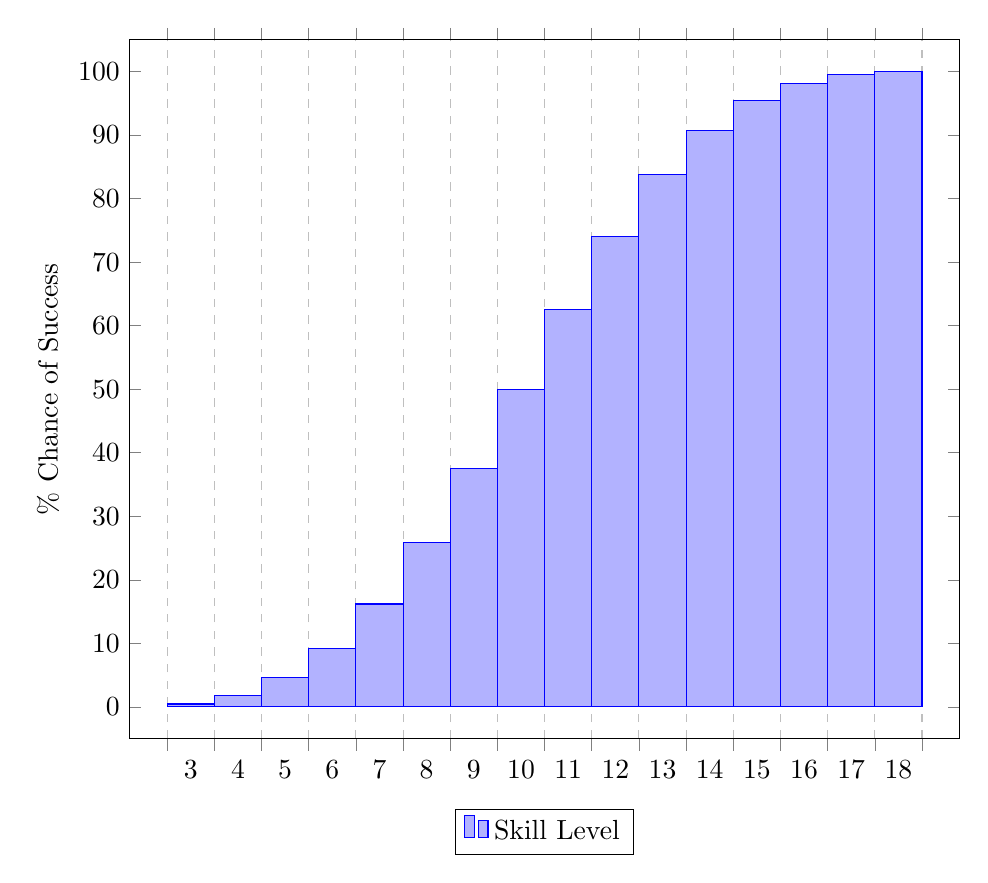
\begin{tikzpicture}
\begin{axis}[
	x tick label style={/pgf/number format/1000 sep=},
	ylabel=\% Chance of Success,
	enlargelimits=0.05,
	ytick = {0, 10, 20, 30, 40, 50, 60, 70, 80, 90, 100},
	legend style = {
	    at={(0.5,-0.1)},
	    grid style = dashed,
	    anchor=north,legend columns=-1
	},
	ybar interval = 1,
]
\addplot 
	coordinates {
	    (3,    0.46) 
	    (4,    1.85)
		(5,    4.63) 
		(6,    9.26) 
		(7,   16.20) 
		(8,   25.93) 
		(9,   37.50) 
		(10,  50.00) 
		(11,  62.50) 
		(12,  74.07)
		(13,  83.80)
		(14,  90.74)
		(15,  95.37)
		(16,  98.15)
		(17,  99.54)
		(18, 100.00)
		(19, 0)
	};
\legend{Skill Level}
\end{axis}
\end{tikzpicture}\\
The graph above shows the probability of succeeding a skill roll. If your character has an effective skill of 10, they have a 50\% chance of succeeding that roll. If they have a skill of 12, the chance of success goes up to 74\%.
\section{Critical Miss Table (Melee)}
\begin{center}
\begin{tabular}{r | l}
    \textbf{Roll} & \textbf{Result}\\\hline
    1 & Your weapon turns in your hand, and you hit with the flat side! \\
    2 & Your weapon breaks! \\
    3 & You lose your grip and the weapon flies out of your hand! \\
    4 & You lose your balance, and your turn! \\
    5 & You trip and fall! You have to get up again.\\
    6 & You hit yourself in the arm or leg! (50\% chance of hitting either)\\
\end{tabular}
\end{center}
\paragraph{Note}For \#3, the weapon flies 1d6 squares (50\% chance forward or backward). If it hits someone, it does half damage and lands there.

%% \section{Critical Miss Table (Ranged)}
%% \begin{center}
%% \begin{tabular}{r | l}
%%     \textbf{Roll} & \textbf{Result}\\\hline
%%     1 & Your weapon jams.\\
%%     2 &\\
%%     3 &\\
%%     4 &\\
%%     5 &\\
%%     6 &\\
%% \end{tabular}
%% \end{center}

\section{Weapons} \label{sec:weapons}
\subsection{Melee Weapons}
\begin{center}
\begin{tabular}{c|c|c|c|c|c}
    \textbf{Category} & \textbf{Name} & \textbf{Class} & \textbf{Damage} & \textbf{Damage Type} & \textbf{Range} \\\hline
    Unarmed  & Fists          & Light & d6-2 & Crushing & Close/1\\
             & Feet           & Light & d6-1 & Crushing & Close/1\\\hline
    Medieval & Short Sword    & Light & d6   & Slashing & Close/1\\
             & Long Sword     & Heavy & d6+2 & Slashing & 1 to 2 \\
             & Mace           & Heavy & d6+2 & Crushing & Close/1\\\hline
    Modern   & Baseball Bat   & Heavy & d6+1 & Crushing & Close/1\\
             & Aluminium Bat  & Light & d6+1 & Crushing & Close/1\\
             & Brass Knuckles & Light & d6-1 & Crushing & Close/1\\\hline
    Future   & Beam Sword     & Light & d6+3 & Slashing & Close/1
\end{tabular}
\end{center}

\subsection{Ranged Weapons}
\begin{center}
\begin{tabular}{c|c|c|c|c}
    \textbf{Category} & \textbf{Name} & \textbf{Damage} & \textbf{Damage Type} & \textbf{Accurate Range} \\\hline
    Primitive & Rock        & d6-1  & Crushing & $0.5 \times Shooting + Prof$  \\\hline
    Medieval  & Short Bow   & d6+1  & Piercing & $Shooting + Prof$ \\
              & Long Bow    & d6+2  & Piercing & $2 \times Shooting + Prof$ \\\hline
    Modern    & Pistol      & 2d6+2 & Crushing & 56m \\
              & Shotgun     & 5d6   & Crushing & 3m \\\hline
    Future    & Laser Gun   & 6d6   & Piercing & 66m \\
\end{tabular}
\end{center}
\paragraph{Note} These ranges are for when you want to shoot without a range penalty.
So despite the fact that a pistol can shoot around 1800m, it's incredibly hard to do so.

\section{Armour}
\begin{center}
\begin{tabular}{c|c|c|c}
\textbf{Category} & \textbf{Name}  & \textbf{PD} & \textbf{DR}\\\hline
         Medieval & Learther       & 1 & 1 \\
                  & Half Plate     & 2 & 2 \\
                  & Full Plate     & 4 & 3 \\
                  & Chain Mail     & 1 & 1 \\\hline
           Modern & Summer Clothes & 0 & 0 \\
                  & Winter Clothes & 0 & 1 \\
                  & Kevlar Vest    & 1 & 3 \\\hline
           Future & Polymer        & 4 & 3 \\
\end{tabular}
\end{center}

\chapter{Character Sheets}\label{app:character-sheets}
This Appendix contains some example character sheets as well as an empty one ready for printout.
\includepdf[pages = -]{graphics/character-sheet-example.pdf}
\includepdf[pages = -]{graphics/siren-character-sheet.pdf}
\end{document}

\chapter{Character Progression}\label{chap:char-prog}
\section{Introduction}
Character progression is important in any RPG.
As your character progresses throughout the adventure, they're naturally going to acquire new abilities, and hone existing their skills.

\section{Experience Points}
To let your characters progress, the game uses \textit{Experience Points} (XP).
XP are used for three things:
\begin{enumerate}
\item Buy proficiency bonuses.
\item Buy trait upgrades.
\item Buy new exploits.
\end{enumerate}
The XP cost for each varies depending on what's being bought.

\section{Buying Proficiency Bonuses and Trait Upgrades}
The price of buying a proficiency bonus or trait upgrade is the same:
Each level costs itself in points.
Put differently: going from level 1 to 2 costs 2 points, and going from 7 to 8 costs 8 points.
Naturally, this means that if you want to buy three levels all at once, you have to pay the price of each successive level.

\paragraph{Example} Joyce wants to increase her warrior's \textit{Wisdom}, it's currently at level 2, and she wants to bring it up to level 5.
To make this happen, she needs to pay 12 XP, because she also needs to buy levels 3 and 4, making it $3 + 4 + 5 = 12$ XP.

\section{Buying Exploits}
As exploits can have a profound impact on the way a character is played, these are naturally much more expensive.
Each exploits costs four times the number of exploits already present, or visualised graphically; the first exploit is free, the next costs 4 XP, the next 8, and so on:

\begin{center}
  \begin{tabular}{r|c|l}
    \textbf{Exploit} & \textbf{XP Cost} & \textbf{Calculation}\\\hline
    1st & Free! & $0 \times 4 = 0$ \\
    2nd & 4     & $1 \times 4 = 4$ \\
    3rd & 8     & $2 \times 4 = 8$ \\
    4th & 12    & $3 \times 4 = 12$\\
    5th & 16    & $4 \times 4 = 16$\\
    6th & 20    & $5 \times 4 = 20$\\
  \end{tabular}
\end{center}

\paragraph{Example} Joyce also wants to buy two new exploits for her warrior.
The warrior already has one exploit, and she needs to pay 12 XP to add those extra exploits, since exploit no.\ 2 costs 4, and no.\ 3 costs 8, the total comes up to $4 + 8 = 12$ XP.

\section{Acquiring XP}
Having an XP system wouldn't make much sense if it wasn't also possible to gain more of it.
\textit{Milestones} are used to accomplish this task.
A milestone is a significant moment in the game that creates a natural \textit{break} in the gameplay.
Examples of natural milestones could be completing a mission or a story arc, at the defeat of some villain that your party has been up against, or even simply at the end of a session.
It is entirely up to the GM to distribute XP, and to help with this, milestones are split into three different kinds: minor, significant, and major.

\paragraph{Note} XP is earned individually, not for the entire party.
It makes little sense that the entire party gets the same amount of XP, if Broot the Destroyer goes hunting orcs all by himself.

\subsection{Minor Milestone}
Minor milestones typically occur at the end of a session, or at the end of a minor in-game event.
Minor milestones should give you a chance to re-balance your character and re-word one of your exploits.

Your character gains 1 XP.

\subsection{Significant Milestones}
Significant milestones occur at important in-game events.
It could be that the party finally found the evil wizard's secret lair, or that some moderate challenge has been overcome.
If in doubt, this can also just happen every 2--3 sessions.

Your character gains 2 XP.

\subsection{Major Milestones}
Major milestones occur at events that shake things up a lot.
Things like, killing the main villain, or driving a group of bandits out of town, or perhaps wreaking a significant amount of havoc.
Alternatively, it could also be at the end of a story arc.

Your character gains 4 XP.

\paragraph{Note} It's of course up to the GM how much XP is awarded, this is meant as more of a guide than a hard rule.

\chapter{Magic} \label{chap:magic}
\section{Introduction}
Some campaigns are set in a fantastical world, full of weirdness, improbable events, and of course: magic.
It is said that any technology that is sufficiently advanced, is completely indistinguishable from magic.
For this reason, we define the term \textit{Magic} to be a bit looser than traditionally.
So, whether we're talking beam sword wielding space wizards, battle mages, or even mutated people that gain power from sea slug juices;
if it seems to give super natural powers, it all just falls under this category.

\paragraph{Note} Spells are anything that is channelled through your body, regardless of how.
Whether the powers were given to you, or you were born with them, doesn't matter.

\section{Spells}
In order to cast a spell, it needs to be known to the character using it.
That is to say, it must be available on the character sheet in some capacity---either in the spell section or perhaps even as an item, depending on how the given setting deals with this.
For all intents and purposes, spells are treated like normal skill checks.

In other words, casting a spell requires two things: A skill roll, and---if the setting calls for it---enough mana.
Like all other skills, spells have four different outcomes, but being magic in nature, they act a bit differently from regular skills:
\begin{itemize}
  \item \textbf{Critical Success.} The spell is performed at double strength, at no extra cost.
  \item \textbf{Success.} The spell succeeds as intended.
  \item \textbf{Fail.} The spell is not performed, but MP is still lost.
  \item \textbf{Critical Fail.} The spell backfires at the GM's or the setting's discretion.
\\This could be the spell having negative unforeseen consequences, and/or the loss of MP.
\end{itemize}

\paragraph{Note} It's up to the GM or the setting to determine the difficulty of a spell.
The difficulty would be set as a $\pm$ skill modifier on the given spell.

\subsection{Affecting the Spells}
Spells come in many different forms: utility, healing, hurting, elemental, bionic etc.
Every spell has an associated mana cost, which consumes a bit of your total mana on each use (see Section~\ref{sec:mana}).

It's up to the players and the GM to decide the kinds of spells that exist within the game, and whether they're too game breaking or not.
Spells can be cast in four different ways:
\begin{enumerate}
  \item On yourself.
  \item Around you.
  \item Away from you.
  \item On someone else.
\end{enumerate}
Depending on the exact nature of that spell, these four casting methods can have vastly different effects, or even be unavailable altogether.

\paragraph{Example} Casting a shield spell on yourself grants you protection.
Casting it around you creates a bubble around you that can shield yourself and your friends.
While casting it away from you can create a wall to shield something/someone further away.

\section{Mana (MP)}\label{sec:mana}
Every character has a mana pool $Int \times Wis$ in size, which represents the amount of magical potential your character can tap into without straining themselves.
In other words, if your character has 5 Int, and 6 Wis, they have 30 Mana Points (MP).
Every spell has an associated mana cost, and using it drains the mana pool accordingly.

\subsection{Running Out of Mana}
When you run out of mana, your can still cast spells!
However, instead of draining mana, your character will instead accumulate 2 Fatigue Points (FP) for every point of mana attempted to use.

\subsection{Regaining Mana}
Mana is regained automatically over time.
About one point every 30 in-game minutes while not at rest,
a point every 10 minutes while relaxing,
and a full restoration after a good night's sleep.

If the setting allows it, mana potions can also help restore some of the spent mana.

\section{Acquiring New Spells}
You can cast any spell your character would logically be acquainted with within the boundries of the setting.
It is, however, up to the GM to decide the number of spells you are allowed to start out with.
Spell familiarity is determined through the skill proficiency system, see Chapter~\ref{chap:skills} for more info.

By default however, the GM decides the XP cost of any given spell, or whether or not characters have \textit{spell slots} that limit the number of spells held. 
The actual intricacies of how a spell is learned is also up to the GM.

\paragraph{Note} In a setting, where it has been decided by the GM that a scroll needs to be found and read in order to learn a spell.
It is possible for the skill check to learn and/or cast the spell is too difficult for the character's current skill level.
This means, XP need to be dedicated to the given spell in order to properly learn it.

\appendix
\documentclass[a4paper]{book}
\usepackage[utf8]{inputenc}
\usepackage[margin=3cm]{geometry} % For smaller margins
\usepackage{appendix} % For appendix support
\usepackage{tikz, pgfplots} % For the skill outcome graph
    \pgfplotsset{width = \textwidth, compat = newest}
\usepackage{graphicx} % For advanced picture insertion
\usepackage{pdfpages} % For inserting PDFs
\usepackage{multicol} % For supporting multi-columnar tables
\usepackage{tcolorbox} % For coloured info boxes
    \tcbuselibrary{skins}
    \tcbset{colback=brown!10, fonttitle=\scshape}
\usepackage{textcomp} % For the interrobang
\usepackage[sc,sf,bf]{titlesec} % for custom titles
\usepackage{sectsty} % for section styles
\usepackage{fancyhdr} % for "fancy" headers
\usepackage[notmath]{sansmathfonts} % for a sans-serif small-caps font
\usepackage{enumitem} % for finer control over enumerations
 
%%%%%%%%%%%%%%%%%%%%%%%%%%%%%%%%%
%% CHAPTERS & SECTION HEADINGS %%
%%%%%%%%%%%%%%%%%%%%%%%%%%%%%%%%%


% Simplifies chapter titles
% No longer says
% Chapter 2
% Game Creation
% but instead simply
% 2 Game Creation
\titleformat{\chapter}[hang]
{\sffamily\bfseries\scshape\Huge}
{\thechapter\quad}{0pt}{}{}

% Removes unnecessarily large margin above chapter title
\titlespacing*{\chapter}{0pt}{-\topskip}{40pt}

% Set the remaining titles to be sans serif and small caps
\allsectionsfont{\sffamily\scshape}

%%%%%%%%%%%%%%%%%
%% THUMB INDEX %%
%%%%%%%%%%%%%%%%%

\renewcommand{\chaptermark}[1]{\markboth{\textsc{\thechapter\ #1}}{}}

%%%%%%%%%%%%%%%%%%%%%%%
%% CUSTOM TEXT BOXES %%
%%%%%%%%%%%%%%%%%%%%%%%
\newtcolorbox{note}{
    enhanced, % enable advanced settings
    left = 10mm, % pushes text away from the left edge by 10mm
    sharp corners, % disables rounded corners
    rounded corners = southeast, % "round" the bottom right corner
    arc is angular, % make the "round" corner an angle
    arc = 3mm, % controls corner cut
    boxrule=0.6pt, % sets box line thickness
    underlay={%
        \path[fill=tcbcolback!80!black] ([yshift=3mm]interior.south east)--++(-0.4,-0.1)--++(0.1,-0.2); % triangle
        \path[draw=tcbcolframe,shorten <=-0.05mm,shorten >=-0.05mm] ([yshift=3mm]interior.south east)--++(-0.4,-0.1)--++(0.1,-0.2); % triangle edge
        \path[fill=gray!50!black,draw=none] (interior.south west) rectangle node[brown!10]{\Huge\bfseries \textinterrobang} ([xshift=8mm]interior.north west);
    },
    drop fuzzy shadow % adds drop shadow
}

\newtcolorbox{example}{
    enhanced,
    title = Example,
    before upper={\parindent15pt\noindent} % add paragraph indentation
}

\title{Siren - Simple RPG Engine $\beta1.0.1$}
\author{By Niko Lepka}
\date{\today}

\begin{document}

\maketitle

\chapter*{Preface}
\section*{What is Siren?}
Siren, the \textbf{Si}mple \textbf{R}PG \textbf{En}gine, is an RPG system that aims at being simple and easy to learn without also compromising on the expressiveness of the system.

An RPG engine, much like a video game engine, is a framework on which you can build your own system. If any of the rules in this seem like they don't \textit{quite} fit what you need, you're free to change them for your campaign

\section*{What are RPGs?}
Role Playing Games, or RPGs for short, are games in which you take the role of some character and act in their stead.
You may know this from video games, where you play some adventurer in a medieval land full of magic and dragons; or where you play a person that's trying to survive in a nuclear wasteland, fighting mutants and warring factions.
But RPGs date back before that.

Traditional RPGs, also known as \textit{Tabletop RPGs} or \textit{Pen and Paper RPGs} date back to the early 1970s.
It's a social game played with a group of friends around a table, mutually telling a common story of great adventure, mysticism, space warfare or whatever they can come up with.

\section*{Who is this for?}
Some role-playing systems have hundreds of books and rules, so many so that it's hard to remember them all, and valuable playtime is spent looking up rules. 
While other systems have so few and vague, that a lot of playtime is spent arguing about which rules apply to a given situation.

Siren is made for those players who wish to have a small yet precise set of rules that can be used in every type of story, whether it's a grand space opera, or high fantasy, Siren's got you covered.

\section*{Conventions}
This book uses standard RPG dice notation, which looks like this: $AdX\pm L$, where $A$ is the number of dice, $X$ is the number of faces on the die, and $L$ is the value added or subtracted after the roll, so $3d6+8$ means roll three six-sided dice, and add 8 to the result.
\paragraph{Note} Notes are displayed like this, and often convey important information to the player or GM regarding a certain mechanic.
\paragraph{Example} Examples are displayed like this, and show a situation in which something is used.

\newpage
\section*{Special Thanks}
Special thanks to the lovely individuals who've helped out with the project:
\begin{center}
    \begin{tabular}{cccc}
        Aleksander Øglænd & Christian J. Martinsen & Marco L.L. Olsen & Morten M. Rasmussen \\
        Patrick A. & Thomas G. McCollin \\
    \end{tabular}
\end{center}

\section*{Licence}
This work is licensed under the Creative Commons Attribution-ShareAlike 4.0 International License.
To view a copy of this license, visit http://creativecommons.org/licenses/by-sa/4.0/ or send a letter to Creative Commons, PO Box 1866, Mountain View, CA 94042, USA.

\tableofcontents

\chapter{Getting Started}
\section{What You Need}
\begin{enumerate}
    \item \textbf{Three to six players.} One of which will have to be the Game Master (GM).
    \item \textbf{Character sheets.} One per player. Additional paper is encouraged, but nor required.
    \item \textbf{GM sheet.} Special sheet for the Game Master.
    \item \textbf{Dice!} At least 3d6 per player, more is not necessarily required, but encouraged.
\end{enumerate}

\subsection{What's a Game Master?}
The Game Master is the special player in a game that directs the flow of the adventure.
The GM is responsible for narrating, setting up obstacles, and role-playing the Non-Player Characters (NPCs) that the players have to face throughout their adventures.

As a GM, the world is at your discretion. 
You roll the dice for everyone that isn't controlled by the players, you set the tone and mood of the environment, and you create the scenarios that will shape the decisions of the players.
You also get to set the difficulty of the obstacles at hand.

\subsection{The Role of the Player}
The player's role is to play their character, and face the trials imposed by the GM.
As a player, you control one of the protagonists in the story that the GM is telling, you make their choices and roll their dice to see how well they perform certain tasks.

\section{Character Sheet}

\section{Performing Actions}
Actions are what usually drives the plot in an RPG, whether it's talking to an NPC or performing great heroic feats, it's all actions.

Some actions have a chance of failure, and thus require you to roll your dice (typically 3d6) to see if you succeed or not. 
These are performed as \textit{Skill Rolls} and are covered more in depth in chapter \ref{chap:skills}. 
The success or failure of this roll decides the fate of your character.

Other actions succeed automatically, and do not require a skill roll, unless there's a very good reason that there should be.
Imagine having to roll your dice every time you wanted to talk to an NPC or walk down the street. 
Unless your character has crippling social anxiety or completely lacks a balance, it's assumed that these sorts of things are automatically successful.
\chapter{Game Creation}
\section{Telling a Story Together}
First and foremost, the point of playing an RPG is telling a story together, how you manage to go about doing so is completely up to you.
Creating a good story for your players to interact with can be a bit difficult at times, but it is absolutely doable.
Let your imagination run wild and see what you can come up with!
Generally speaking you need a few things:
\begin{itemize}
    \item A setting
    \item A scale
    \item A plot-line
    \item NPCs
\end{itemize}

\section{Setting}
The setting is one of the most important aspects of your game.
It determines everything from whether or not magic exists, to things like alien races, or level of technology.

Do you want to make 1940's style Noir story set in the distant future in a city that spans an entire planet? Go for it!
The most important thing, is that you---as the GM---can keep track of the setting, and keep it somewhat consistent.
Consistency is important so that things don't feel out of place. 
Don't be afraid to break consistency if you want to surprise or weird your players out.
It's your game world, make it however you want it.

\section{Scale}
When creating a game, it's also important to keep the scale of it all in mind.
Do you want a giant flourishing world filled to the brim with characters and opportunities on every corner? 
Or do you instead want something small and personal that can be wrapped up in a few sessions, but leaves a deep and profound impact on the players?
It's all up to you.
Just remember not to bite over more than you can chew.
It's easy to create this massive world and get lost in it.

\section{Plot}
What is a story without issues to resolve? Like any good movie or video-game, the story needs a plot-line.
Is a big evil corporation trying to take over the world?
Is a secret society conspiring against the general population?
Maybe a hoard of dragons are stealing all the magic in the world for themselves in preparation for an upcoming war.

It's up to you, make it good.

\section{Non-Player Characters}
What is a world if there aren't anyone in it?
Just like the players need characters, so does the game world.
It's important to remember not only to make major plot-related NPCs, like an spy in the organisation you're trying to infiltrate, or the big bad guy that is foiling your plans at every step.
But minor NPCs like the slew of goons you want your players to fight, or that one one-off clerk at the shop that the players want to interact with.

NPCs generally come in those two flavours: Major and Minor.
Major NPCs are best created with a full character sheet, like the players, but minor NPCs can make by with just the most important stats written down.
\chapter{Character Creation}\label{chap:char-creat}
\section{Introduction}
Character creation is perhaps one of the most important aspects of an RPG.
How you design your character impacts how the game is going to be played.
This chapter is meant as a guide to help you through creating your character in Siren. 
Appendix~\ref{app:character-sheets} has a blank character sheet for you to copy.

\begin{note}
    All fractions are rounded down by default unless explicitly stated otherwise.
\end{note}

\section{Use Your Imagination}
Make your character yours.
Think of a back-story for them, give them a reason to exist in the world you're playing in.
If you are unsure about what works in the setting, ask your GM for help; after all, they're the one curating the game.
Work with the GM and the other players to create a character that best works for your game.

\begin{note} 
    The following is meant as a loose guide.
    If the GM decides, any and all of the rules below can be changed to suit your particular game.
\end{note}

\section{The Character Sheet}
The character sheet comes in three pages.
\paragraph{Page 1} The general stats page, which contains your traits, skills, and exploits.
\paragraph{Page 2} The weapons, spells, and armour page, which keeps track of your weapons, spells, armour, and shields.
\paragraph{Page 3} The character and possessions page, which keep track of your character notes (back-story, etc.), money, and loot.
Example character sheets have been included in Appendix~\ref{app:character-sheets}.

\begin{note} 
    In case you can't fit on everything on the character sheet, feel free to use the reverse side of the paper!
\end{note}

\section{Building a Character}
\subsection{Experience Points (XP)}
To help you out, you'll get \textbf{35 XP} to start out (The GM may decide to give more or less XP depending on setting or circumstance).
These can be used to purchase skill specialisations and upgrade your traits if you so desire at the beginning of the game.
Check Chapter~\ref{chap:char-prog} for more information about how XP works.

\subsection{Traits}
During character creation, each trait level costs 1 XP and cannot exceed a trait level of 10.

The derived traits are calculated like this:
\begin{center}
\begin{tabular} {r | l} 
\textbf{HP:} & $Con \times 2$ \\
\textbf{FP:} & $Con + Str$ \\
\textbf{MP:} & $Int \times Wis$ \\
\textbf{Speed:} & $Athletics / 2$\\
\textbf{Parry:} & $Fighting / 2 + \mathit{DfM}$\\
\textbf{Dodge:} & $Speed + \mathit{DfM}$ \\
\end{tabular}
\end{center}
See Section~\ref{sec:skills-in-depth} for Athletics, and Section~\ref{sec:defence} for an explanation on \textit{Parry}, \textit{Dodge}, and \textit{DfM}.

\begin{note} 
    The \textit{Parry} box on the character sheet is split in two, this is due to the fact that there are \textit{two} parry traits: one for \textit{Fighting (Heavy)} and one for \textit{Fighting (Light)}.
    It is up to you which half to use for which, as long as you can remember it.
\end{note}

\begin{example}
A character with the traits set up like this:

\begin{center}
    \begin{tabular}{ccccccc}
        \textbf{Agi} & \textbf{Cha} & \textbf{Con} & \textbf{Dex} & \textbf{Int} & \textbf{Str} & \textbf{Wis} \\\hline
        6 & 4 & 4 & 6 & 5 & 4 & 3\\ 
    \end{tabular}
\end{center}
Would cost 32 XP to build.
Note that a value of 5 is considered \textit{average}.

See Appendix~\ref{app:character-sheets} for an example character with these exact traits.
\end{example}

\subsection{Skills}
Calculate your character's skills based on their traits as shown in the skill listing on your character sheet.
Think about what your character is particularly good at, these skills can be what your character specialises in.
See Chapter~\ref{chap:skills} for more information about Skills in general.

\subsection{Exploits}
Exploits are entirely player-defined, and are a way of personalising your character to fit your play-style.
Exploits can range from simply providing bonuses, to providing exceptions to the existing rules.
You can read more about exploits in Chapter~\ref{chap:exploits}.

\subsection{Weapons}
The weapons section of the character sheet lists all the relevant attributes of a given weapon.
The section is divided into five columns: \textit{name}, \textit{specialisation}, \textit{damage \& type}, \textit{range}, and \textit{parry}.

\paragraph{Name} The given name of the weapon, this could be something as simple as ``Long Sword'' ``Glock~22'' to something as personal as ``Widow-Maker'' or ``Demon Slayer''.

\paragraph{Specialisation} The name of the given specialisation the weapon falls under.
The idea is that, if you're able to use one long sword, you're able to use all of them, doesn't matter if one has a fancier handle than the other. 
The specialisation is also what you upgrade if you want to be better at using the weapon.
You can think of this as the \textit{weapon class}.

\paragraph{Damage \& Type} The dice you roll and the type of damage it deals.
Examples include $2d6\ \mathit{Piercing}$ and $1d6+3\ \mathit{Crushing}$.

\paragraph{Range} The range of the weapon in meters.
The range of a weapon is most useful when playing with a game mat (see Chapter~\ref{chap:combat}), where the width of each square corresponds to $1m$.

\paragraph{Parry} The individual weapon's parry score, which differs from the score in the box on the front of the character sheet.
It is included here for quick reference.

This is the \textit{Parry} score from the first page, plus the weapon's specialisation.

\subsection{Shields \& Armour}
The shields and armour sections list the relevant attributes of your characters' defensive equipment.
Where they differ, is in the fact that shields can be used offensively as well as defensively.
Shields share all columns as weapons except range, as all shields are considered close-range weapons.
Therefore, refer to the relevant columns in the weapons section above.

The defensive stats for shields and armour are divided into \textit{DfM} and \textit{Damage Resistance}.
Refer to Section~\ref{sec:defence} for more info.

\paragraph{DfM} Short for \textbf{D}e\textbf{f}ence \textbf{M}odifier.
It is a type of passive bonus applied to your \textit{Dodge} and \textit{Parry}, which makes it more likely for you to not get hurt during combat.

\paragraph{Damage Resistance} Provides damage reduction in the case you \textit{do} get hit.
Damage Resistance makes attacks hurt less, thus increasing your survivability during combat.

\subsection{Spells}
The spell section lists the spells your character knows and is able to use.
The section is divided into \textit{name}, \textit{cost}, and \textit{description}.
Check Chapter~\ref{chap:magic} for more information about magic in general.

\paragraph{Name} The name of the spell.
Unlike weapons, spells don't fall into general categories in quite the same way, so specialisations need to be handled on a per-spell basis.
It's important to note, that just because your character doesn't specialise in a given spell, it doesn't also mean they can't use it.
It is ultimately up to the GM to decide whether a spell can be learned or not.

\paragraph{Cost} The cost of the spell in $MP$.
Some spells consume mana-points, which limit the number of times a spell can be used.
See Section~\ref{sec:mana} for more details.

\paragraph{Range} The range of the spell.
Depending on the setting, the range of any given spell can vary widely from point-blank to several kilometres.

\paragraph{Description} Describes the effects of the spell in question.
Things like how it behaves and---if applicable---how much damage it deals.

\subsection{Equipment}
The equipment section lists all the stuff you're carrying.
This is everything from armour and clothes, to loot, to weapons.

\subsection{Money}
Each box in the money section is for the type of the currency carried, and the lines next to the boxes are meant for the amount of said currency.
So if you're playing an international spy, the boxes could hold \textit{USD}, \textit{GBP}, \textit{EUR}.
And if you're playing in a fantasy setting, they could hold \textit{Gold}, \textit{Silver}, \textit{Bronze}.

\begin{example} 
Here's an example of how the money table on the character sheet could be filled in a medieval fantasy setting:
\begin{center}
    \begin{tabular}{|r|l@{\hspace{1cm}}}\cline{1-1}
        Platinum & 0\\\hline
        Gold & 12\\\hline
        Silver & 144\\\hline
        Copper & 59\\\hline
               & \\\hline
    \end{tabular}
\end{center}
\end{example}
\section{Adding or Changing Traits}
Your setting may not be satisfied with just the seven basic traits included in the core rules.
It could be that you feel it would be better with an eighth trait like \textit{Faith} or \textit{Psionics} or something else entirely.
Maybe you instead prefer combining some of the traits into broader categories, like combining \textit{Int} and \textit{Wis} into a joined \textit{Mental} trait.
It's all doable, should you want to do so.
Just keep in mind: it's easier to add traits than to remove or combine them, since the latter will inevitably require you to rewrite many of the \textit{Skills} to fit the new listing.
\chapter{Skills} \label{chap:skills}
\section{Introduction}
Skills are the primary workhorse in the game. 
Whenever there's any situation that requires action, a player rolls against their skill plus/minus modifier. 
There are 18 different skills, as seen in figure \ref{fig:skills}. 
These skills reflect the different types of actions a player can perform during play.


\section{Skill Rolls}
The player rolls three six-sided dice (3d6) against their skill of choice, if the outcome is $\leq$ the skill level, it's a success, if not, it's a fail.
Rolling a 3, is an automatic success (regardless of level), and rolling an 18 is an automatic fail (also regardless of level).

\paragraph{Example} Say Alice wants to persuade a guard to do something stupid. Her \textit{Persuasion} skill is at 13. 
She rolls 3d6, and rolls a 1, a 5, and a 3, which is 9 in total. This means she successfully persuades the guard.

\begin{figure}
\centering
\begin{tabular}{r | c | c | l}
\textbf{Category} & \textbf{Skill}   & \textbf{Traits} & \textbf{Description} \\\hline
    Mental    & Academics        & $Int+Int$ & Use vast knowledge of a certain field.        \\
              & Investigation    & $Int+Wis$ & Searching for things and information.         \\
              & Magic            & $Int+Wis$ & Perform fantastical feats.                    \\
              & Perception       & $Int+Wis$ & The passive ability to spot things.           \\
              & Survival         & $Con+Int$ & Surviving in certain environments.            \\
              & Thievery         & $Dex+Int$ & Performing certain larcenous activities.      \\\hline
    Physical  & Athletics        & $Agi+Con$ & Perform a certain task that requires stamina. \\
              & Fighting (Heavy) & $Agi+Str$ & The ability to fight with heavy weapons.      \\
              & Fighting (Light) & $Agi+Dex$ & The ability to fight with light weapons.      \\
              & Physique         & $Con+Str$ & Any action that requires strength.            \\
              & Stealth          & $Agi+Wis$ & Sneaking around and acting unseen.            \\\hline
    Social    & Contacts         & $Cha+Int$ & Make and use connections with people.         \\
              & Insight          & $Cha+Wis$ & Sensing and social cues and motivation        \\
              & Nursing          & $Cha+Wis$ & Taking care of people                         \\
              & Persuasion       & $Cha+Wis$ & Manipulating people.                          \\\hline
    Technical & Crafting         & $Dex+Int$ & Making things with your hands.                \\
              & Shooting         & $Dex+Wis$ & Shooting or throwing objects.                 \\
              & Vehicle (Air)    & $Dex+Wis$ & Operating motorised air vehicles.             \\
              & Vehicle (Land)   & $Dex+Wis$ & Operating motorised land vehicles.            \\
              & Vehicle (Sea)    & $Dex+Wis$ & Operating motorised sea vehicles.             \\
\end{tabular}
\caption{Skill Listing}
\label{fig:skills}
\end{figure}
\newpage
\section{Proficiency \& Specialisation}
Your character can specialise in any number of different skills.
Specialising grants the skill a \textit{Proficiency Bonus} of $+3$ to that particular specialisation.

\paragraph{Note} Just because your character hasn't specialised in anything, does not mean they cannot perform it, it just means they don't get the proficiency bonus.

\paragraph{Example} Joyce is an Olympic runner, and has a \textit{Constitution} of 5, and an \textit{Agility} of 5; this gives her an \textit{Athletics} score of 10. 
As a runner, she specialises in running, which grants her a $+3$ bonus to her \textit{Athletics} roll whenever she needs to perform a running task.
She rolls 11, but because her effective \textit{Athletics} score is 13 due to the bonus, she succeeds.

\newpage
\section{Skills in Depth}
\subsection{Mental Skills}
\subsubsection{Academics (Int + Int)}
The Academics skill, called \textit{Knowledge}, or \textit{Lore} in other games, is the skill of knowing things factually. 
This can be things your character has read, or something they've researched.
If your character needs to identify ancient writing, source herbs, design circuits, or have a meaningful discussion with an expert, this is the go-to skill.

\paragraph{Specialisations:}
\begin{center}
    \begin{tabular}{c|c|c|c}
        Maths & Physics & Chemistry & Theology \\
        Medicine & Literature & Linguistics & History \\
        Anthropology & Computer Science & Magic & Botany \\
        Geology & Astronomy & Quantum Physics & Computer Security \\
    \end{tabular}
\end{center}

\subsubsection{Investigation (Int + Wis)}
Investigation is the skill of actively searching for things and gathering information.
Whether your character is hunting for clues or digging through books, investigation is the skill to use.

\subsection{Magic (Int + Wis)}
Magic is the skill of performing fantastical things with power channeled through the body.
Whether it's chi energy, spiritual power, nanobots, genetic modification, or the essence of the universe that powers your abilities, it all falls under \textit{Magic}.

\paragraph{Specialisations:}
\begin{center}
  \begin{tabular}{c|c|c|c}
    Life & Construction & Destruction & Utility \\
    Earth & Water & Air & Fire \\
    Arcane & Black/Dark & White/Light & Temporal \\
    Divine & Diabolic
  \end{tabular}
\end{center}
Magic is covered much more in depth in chapter \ref{chap:magic}.

\subsubsection{Perception (Int + Wis)}
Perception, called things like \textit{Notice} or \textit{Awareness} in otehr games, is the skill of using your senses to \textit{passively} notice what's going on around you.

\subsubsection{Survival (Con + Int)}
Survival is the skill of surviving; particularly in inhospitable environments.

\paragraph{Specialisations:}
\begin{center}
    \begin{tabular}{c|c|c|c}
        Desert & Tundra & Jungle & Island \\
        Prairie & Urban & Off-World & Space \\
        Under Water & Underground & Mountain & Arctic \\
    \end{tabular}
\end{center}

\subsubsection{Thievery (Dex + Int)}
Thievery is a catch-all term for general larcenous and/or criminal skills that (generally) involve thought and finesse.
These skills are regarded as such regardless of their actual use.

\paragraph{Specialisations:}
\begin{center}
    \begin{tabular}{c|c|c}
        Pick-Pocket & Lock-Pick & Sleight of Hand \\
        Alarm Deactivation & Hacking & Evidence Tampering \\
    \end{tabular}
\end{center}

\subsection{Physical Skills}
\subsubsection{Athletics (Agi + Con)}
Athletics, sometimes called \textit{Endurance} in other games, is a skill that has your character perform physically challenging things, often involving swiftness or stamina.
Tasks such as running, climbing, or swimming fall under here.

\paragraph{Specialisations:}
\begin{center}
    \begin{tabular}{c|c|c|c}
        Running & Climbing & Swimming & Jumping \\
        Acrobatics & Biking & Diving & Sailing \\
    \end{tabular}
\end{center}

\paragraph{Note} Sailing here refers to sailing a non-motorised sail or row boat. For motorised sailing, see the skill \textit{Driving}.

\subsubsection{Fighting (Heavy) (Agi + Str)}
This is the skill of melee fighting with heavy weaponry. Weapons such as clubs, mallets, war-hammers, axes, etc. fall under this skill.

\paragraph{Specialisations:}
\begin{center}
    \begin{tabular}{c|c|c|c}
        Mace & Club & Mallet & War Hammer \\
        Claymore & Baseball Bat & Pipe & Pipe Wrench \\
        Battle Axe & Two-by-Four & Odachi & Talwar \\
    \end{tabular}
\end{center}

\subsubsection{Fighting (Light) (Agi + Dex)}
This is the skill of melee fighting without weapons or wit light weaponry. 
Weapons such as rapiers, short swords, lances, and knives fall under here.

\paragraph{Specialisations:}
\begin{center}
    \begin{tabular}{c|c|c|c}
        Rapier & Short Sword & Katana & Beam Sword \\
        Knife & Ice Pick & Baton & Brass Knuckles \\
        Fist (punching) & Foot (kicking) & Rolling Pin & Letter Opener \\
    \end{tabular}
\end{center}

\subsubsection{Physique (Con + Str)}
Physique, the raw strength counterpart to Athletics. 
This skill involves everything that requires strength.
Lifting, pulling, or pushing heavy objects are things that fall under here.

\subsubsection{Stealth (Agi + Wis)}
Stealth is the act of moving around unnoticed.
Tasks such as blending in, sneaking, and infiltrating all fall under here.

\subsection{Social Skills}
\subsubsection{Contacts (Cha + Int)}
Contacts is the skill of creating, maintaining, and making use of contacts.
So if your character needs to call a friend for help, or establishing a new connection with someone for use later, this is the skill for you.

\subsubsection{Insight (Cha + Wis)}
Insight, called \textit{Sense Motive} or \textit{Empathy} in other games, is the dual/opposite of \textit{Persuasion}. 
This skill is all about reading people and their intentions, and trying to figure out what they're up to.
So if you're suspecting a salesman is trying to scam you, or if you're trying to figure out if an unstable inmate is about to have a wild mood swing, this is the go-to skill.

\subsection{Nursing (Cha + Wis)}
The Nursing skill is all about taking care of animals and people and making them feel good.
A good nurse can have a positive effect on someone's mental and physical health, and in fact can help speed up their natural healing.

\subsubsection{Persuasion (Cha + Wis)}
Persuasion is the skill for manipulating people for good or bad.
Whether you need to lure a guard away from his post, trick the evil sorcerer to reveal his secret plan, or strike a favourable deal with the mob boss, or maybe you just want to sit around in a pub cracking jokes, lightening the mood of the people around; this is the skill you want to use.

\paragraph{Specialisations:}
\begin{center}
    \begin{tabular}{c|c|c|c}
        Bargaining & Charming & Convincing & Inciting \\
        Seducing & Taunting & Provoking & Distracting \\
        Rapport & Deception & Bluffing & Intimidation
    \end{tabular}
\end{center}

\subsection{Technical Skills}
\subsubsection{Crafting (Dex + Int)}
The skill of making things, any hobby or task that involves producing something tangible with your hands belongs here.

\paragraph{Specialisations:}
\begin{center}
    \begin{tabular}{c|c|c|c}
        Paper Crafts & Origami & Carpentry & Woodworking \\
        Masonry & Smithing & Machining & Electronics \\
        Gadgeteering & Knitting & Casting & Sculpting \\
    \end{tabular}
\end{center}

\subsubsection{Vehicle, Air (Dex + Wis)}
The act of operating an airborne vehicle.

\paragraph{Specialisations:}
\begin{center}
    \begin{tabular}{c|c|c|c}
        Plane & Jet & Helicopter & Hot Air Balloon \\
        Commercial Liner & Zeppelin & Flying Car \\
    \end{tabular}
\end{center}

\subsubsection{Vehicle, Land (Dex + Wis)}
The act of operating land vehicles.

\paragraph{Specialisations:}
\begin{center}
    \begin{tabular}{c|c|c|c}
        Car & Truck & Tractor & Tank \\
        Train & Moped & Motorcycle & Hovercraft
    \end{tabular}
\end{center}

\subsubsection{Vehicle, Sea (Dex + Wis)}
The act of operating water based vehicles.
Note that sailing sail/row boats are Olympic disciplines, and thus fall under \textit{Athletics}.

\paragraph{Specialisations:}
\begin{center}
    \begin{tabular}{c|c|c|c}
        Jet-Ski & Motor Boat & Yacht & Cruise Liner \\
        Submarine & Hovercraft & 
    \end{tabular}
\end{center}

\subsubsection{Shooting (Dex+Wis)}
Shooting is the skill of launching projectiles, whether it be by throwing, or launching them from a device.

\paragraph{Specialisations:}
\begin{center}
    \begin{tabular}{c|c|c|c}
        Throwing & Slingshot & Bow & Crossbow \\
        Pistol & Revolver & SMG & Rifle \\
        Assault Rifle & Cannon & Ballista & Trebuchet \\
        Mortar & Tank Turret & Helicopter Turret & Blowpipe
    \end{tabular}
\end{center}

\newpage
\section{Contest of Skills}\label{sec:contest}
Situations arise, when your character needs to test their skills and prove their worth, this is done via a \textit{Contest of Skills}.
These contests come in three different variants: \textit{Passive}, \textit{Active}, and \textit{Tournament}.

\subsection{Passive Contest}
A passive contest arises when the character needs to overcome some passive obstacle. This could be things like walking a tightrope, picking a lock, leaping over a gap, etc.
The GM silently decides the level of difficulty by announcing a skill +/- a modifier that needs to be rolled.

\paragraph{Example} Astrid is running from her pursuers across the rooftops of ancient Rome, she needs to clear a particularly wide gap between the buildings. Astrid says \textit{``I'm jumping the gap''}, to which the GM replies \textit{``Roll Athletics -2''}. Astrid's Athletics skill is at 11, at -2, she must roll 9 or less to succeed. She rolls an 8 and gracefully leaps between the buildings.

\subsection{Active Contest}
An active contest is when the character is up against someone or something that actively works against them. Be it trying to pick-pocket a guard, an intense sword-fight, or playing chess against an opponent; all of this providing an \textit{active} resistance.

In an active contest, both parties roll against their most applicable skill, the outcome is judged as follows:

\begin{center}
    \begin{tabular}{c|c|c}
    \textbf{Character A} & \textbf{Character B} & \textbf{Winner}\\\hline
    Fail & Fail & The one failing by least \\
    Fail & Success & Character B \\
    Success & Fail & Character A \\
    Success & Success & The one succeeding by most
    \end{tabular}
\end{center}
If no one fails or succeeds more than the opponent, re-roll.

\paragraph{Example} Tom wants to sneak past a guard, Tom's \textit{Stealth} is at 9, he rolls 11, failing by 2 degrees. 
The guard's \textit{Perception} is at 10, but rolls 13, failing by 3 degrees. 
Tom failed less than the guard, thus successfully sneaking past the guard.

\subsection{Tournaments}
Tournaments are \textit{longer} contests of skills.
Tournaments are divided into rounds, whoever wins the most rounds wins the tournament.
Each individual round is a regular \textit{active contest}.

\chapter{Example Exploits}
Trying to come up with new exploits in the heat of the moment can be hard.
This appendix exists to alleviate this pain and get the proverbial juices flowing.

\section{Red Tape Recorder}
Persuasion is $Int + Int$ when dealing with government officials.
\chapter{Magic} \label{chap:magic}
\section{Introduction}
Some campaigns are set in a fantastical world, full of weirdness, improbable events, and of course: magic.
It is said that any technology that is sufficiently advanced, is completely indistinguishable from magic.
For this reason, we define the term \textit{Magic} to be a bit looser than traditionally.
So, whether we're talking beam sword wielding space wizards, battle mages, or even mutated people that gain power from sea slug juices;
if it seems to give super natural powers, it all just falls under this category.

\paragraph{Note} Spells are anything that is channelled through your body, regardless of how.
Whether the powers were given to you, or you were born with them, doesn't matter.

\section{Spells}
In order to cast a spell, it needs to be known to the character using it.
That is to say, it must be available on the character sheet in some capacity---either in the spell section or perhaps even as an item, depending on how the given setting deals with this.
For all intents and purposes, spells are treated like normal skill checks.

In other words, casting a spell requires two things: A skill roll, and---if the setting calls for it---enough mana.
Like all other skills, spells have four different outcomes, but being magic in nature, they act a bit differently from regular skills:
\begin{itemize}
  \item \textbf{Critical Success.} The spell is performed at double strength, at no extra cost.
  \item \textbf{Success.} The spell succeeds as intended.
  \item \textbf{Fail.} The spell is not performed, but MP is still lost.
  \item \textbf{Critical Fail.} The spell backfires at the GM's or the setting's discretion.
\\This could be the spell having negative unforeseen consequences, and/or the loss of MP.
\end{itemize}

\paragraph{Note} It's up to the GM or the setting to determine the difficulty of a spell.
The difficulty would be set as a $\pm$ skill modifier on the given spell.

\subsection{Affecting the Spells}
Spells come in many different forms: utility, healing, hurting, elemental, bionic etc.
Every spell has an associated mana cost, which consumes a bit of your total mana on each use (see Section~\ref{sec:mana}).

It's up to the players and the GM to decide the kinds of spells that exist within the game, and whether they're too game breaking or not.
Spells can be cast in four different ways:
\begin{enumerate}
  \item On yourself.
  \item Around you.
  \item Away from you.
  \item On someone else.
\end{enumerate}
Depending on the exact nature of that spell, these four casting methods can have vastly different effects, or even be unavailable altogether.

\paragraph{Example} Casting a shield spell on yourself grants you protection.
Casting it around you creates a bubble around you that can shield yourself and your friends.
While casting it away from you can create a wall to shield something/someone further away.

\section{Mana (MP)}\label{sec:mana}
Every character has a mana pool $Int \times Wis$ in size, which represents the amount of magical potential your character can tap into without straining themselves.
In other words, if your character has 5 Int, and 6 Wis, they have 30 Mana Points (MP).
Every spell has an associated mana cost, and using it drains the mana pool accordingly.

\subsection{Running Out of Mana}
When you run out of mana, your can still cast spells!
However, instead of draining mana, your character will instead accumulate 2 Fatigue Points (FP) for every point of mana attempted to use.

\subsection{Regaining Mana}
Mana is regained automatically over time.
About one point every 30 in-game minutes while not at rest,
a point every 10 minutes while relaxing,
and a full restoration after a good night's sleep.

If the setting allows it, mana potions can also help restore some of the spent mana.

\section{Acquiring New Spells}
You can cast any spell your character would logically be acquainted with within the boundries of the setting.
It is, however, up to the GM to decide the number of spells you are allowed to start out with.
Spell familiarity is determined through the skill proficiency system, see Chapter~\ref{chap:skills} for more info.

By default however, the GM decides the XP cost of any given spell, or whether or not characters have \textit{spell slots} that limit the number of spells held. 
The actual intricacies of how a spell is learned is also up to the GM.

\paragraph{Note} In a setting, where it has been decided by the GM that a scroll needs to be found and read in order to learn a spell.
It is possible for the skill check to learn and/or cast the spell is too difficult for the character's current skill level.
This means, XP need to be dedicated to the given spell in order to properly learn it.
\chapter{Combat}
\section{Introduction to Combat}
Combat is a staple of most RPGs. 
It's intense, often exhilarating, and it gives the players a chance to strategise. Combat is essentially a series of \textit{Contests of Skill} (see section \ref{sec:contest}), but due to the nature of combat are naturally a bit more involved.
\subsection{Turns}
Combat is split into a number of turns, each turn represents about 6 seconds of in-game time, meaning 10 turns make up an in-game minute.

\paragraph{Note} One turn is the time it takes for every character to have had a go, not the time for each individual character.
\subsection{Turn Order}
To determine turn order, each player rolls $1d6+Athletics$. The turn-order is then ordered highest to lowest. Highest result goes first, lowest goes last. Any ties require a re-roll.

\paragraph{Example} Alice, Bob, and Clarice all roll for turn order. They have an athletics score of 9, 9, and 10 respectively. Alice rolls a 5, Bob rolls 3, and Clarice rolls a 6. Clarice goes first with 16, Alice is next with 14, and Bob is last with a score of 12.

\subsection{Simple Vs. Advanced Combat}
Siren supports two different styles of combat: \textit{simple}, and \textit{advanced}.

Simple combat is the most straightforward, and involves nothing more than your character sheets and your imagination. A drawn map to help visualise the space is nice, but not required.

Advanced combat, on the other hand, uses a battle mat divided into squares. This mat is used to communicate the exact position of characters and NPCs, and helps visualise movement and trajectories on the battlefield.

\subsection{Active Defence}
Active defence differs from the \textit{Defend} action in that it occurs on the attacker's turn.
There are two things a character can do when actively defending:
\begin{enumerate}
    \item \textbf{Dodge.} Roll against your \textit{Move} trait.
    \item \textbf{Parry.} Roll against half of your weapon skill, rounded down.
\end{enumerate}
You get an additional $+2$ to your roll if you also choose to move out of the way of the attack.

\newpage
\section{Simple Combat}

\subsection{Attack (Melee)}
\begin{enumerate}
    \item Roll against the appropriate weapon skill.
    \item If you succeed, the opponent gets to roll active defence.
    \item If the defence fails, roll for damage for the appropriate weapon.
\end{enumerate}

\subsection{Attack (Ranged)}
\begin{enumerate}
    \item Calculate effective skill level.
        \begin{enumerate}
            \item Target is \textbf{close}: Use base-skill.
            \item Target is at \textbf{medium} range: $Skill-3$.
            \item Target is \textbf{far}: $Skill-6$.
            \item Target is \textbf{very far}: $Skill-9$.
        \end{enumerate}
    \item Roll to attack, using the modified skill.
    \item If you succeed, target opponent may roll to dodge.
    \item If the dodge fails, roll for damage.
\end{enumerate}

\subsection{Defend}
Spend your turn doing nothing but defending. 
You get an additional $+2$ to your active defences. 
You may not attack during this turn.

\subsection{Long Action}
Any non-combat task that takes more than one turn is a \textit{long action}.
Examples of long actions could be picking a lock, untying someone, calling for backup, or applying bandages.

\subsection{Prepare Action}
Prepare an action to be triggered at a specific moment.
This can be waiting to hit someone until they're about to draw their sword, waiting for someone to turn around before hitting them in the head, or waiting for your opponent to reload their weapon before casting a spell.

\newpage
\section{Advanced Combat}
Advanced combat is much like simple combat, except it uses a battle mat. Because of this, the different possible actions in a turn are affected by this addition.

\subsection{Movement}
Particularly, the characters rely on their movement points to move about the battle mat.
Movement is 8-directional (see figure \ref{fig:directions}), and moving in any direction costs 1 movement point.

\begin{figure}
    \centering
    \includegraphics{graphics/directions.png}
    \caption{The eight movement directions}
    \label{fig:directions}
\end{figure}

Your character can only move as far as their movement points allow, but you may choose to move a shorter distance if you so desire. Figure \ref{fig:movement} shows an example of a character moving 4 squares, which is worth 4 movement points.

\begin{figure}
    \centering
    \includegraphics{graphics/movement.png}
    \caption{Example of movement.}
    \label{fig:movement}
\end{figure}

\subsection{The Grid}
The battle mat is subdivided into a grid of squares. 
The in-game size of a square is $1m^2$, although the GM may scale it up or down as necessary.
The GM must alert the players of the scale if it differs from the standard $1m^2$.

\subsection{Actions}
\subsubsection{Long Action}

\subsubsection{Move \& Attack (Melee)}
\begin{enumerate}
    \item Move up to half your movement (rounded down) before or after attacking.
    \item Roll against the appropriate weapon skill.
    \item If you succeed, the opponent gets to roll active defence.
    \item If the defence fails, roll for damage for the appropriate weapon.
\end{enumerate}

\subsubsection{Move \& Attack (Ranged)}
\begin{enumerate}
    \item Move up to half your movement (rounded down) before or after attacking.
    \item Calculate effective skill level.
        \begin{enumerate}
            \item If target is within weapon's range, do nothing else.
            \item Subtract 3 points every time you exceed the range.
        \end{enumerate}
    \item Roll to attack, using the modified skill.
    \item If you succeed, the opponent may roll to dodge.
    \item If the dodge fails, roll for damage.
\end{enumerate}

\paragraph{Example} Will the Ranger is out hunting for his party. He spots a deer in the distance. His bow has a range of 100 metres, the deer is 300 metres away. This exceeds the bow's range twice ($2\times -3$ penalty). Will must roll $Longbow-6$ to succeed.

\subsubsection{Move \& Defend}
Move up to half your movement (rounded down) before defending. 
Spend the rest of your turn doing nothing else. 
You get an additional $+2$ to your active defences. 
You may not attack during this turn.

\subsubsection{Prepare Action}
Prepare an action to be triggered at a specific moment.
This can be waiting to hit someone until they step into the square in front of you, waiting for your opponent to reload their weapon before casting a spell, or waiting for a party member to stand in the square next to you before charging at the enemies.

\subsubsection{Relocate}
Move as far as your movement score allows and do nothing else.
Roll \textit{Athletics} to run, this doubles your range if you succeed.
If you fail you trip and fall prone.
If prone you may try to get up again on your next turn.
\chapter{Defence \& Damage Resistance}\label{chap:defence}
\section{Introduction}
Let's face it, taking damage isn't fun, but unfortunately, it's a natural and almost unavoidable consequence of combat.
Luckily, there are ways to avoid, or at least mitigate some of the damage taken.
For this, there are three different things that might help you out: damage resistance, and active and passive defence.

\section{Active Defence}
Active defence (AD), is performed by your character during combat.
This refers to actions like dodging, blocking, or parrying an attack.
More often than not, active defences have a very low chance of success, but also have a very high reward, as they make it possible to completely avoid all damage from an attack.

There are two things a character can do when actively defending:
\begin{enumerate}
    \item \textbf{Dodge.} Roll against your \textit{Speed} trait.
    \item \textbf{Parry.} Roll against half of your weapon skill, rounded down.
\end{enumerate}
You get an additional $+2$ to your roll if you also choose to move out of the way of the attack.

\section{Passive Defence}
Passive defence (PD), is defence gained from your armour.
Generally, thicker armour usually grants a bigger passive defence bonus.
The passive defence is added to your active defence score when performing a defence roll.

\paragraph{Example} Jean has been challenged by a rival clan's champion, who is charging at him, claymore raised high.
Jean's dodge is 6, his leather armour and buckler give him 1 PD each.
Added together, it gives him an effective defence of 8, which he then needs to roll against to evade the foe.
He rolls an 8! He slips right past his opponent, deflecting the claymore with his buckler.

\section{Damage Resistance}
Damage resistance (DR), is something that always applies, whether your character is aware of the attack or not.
Damage resistance is granted by certain armour, shields, and potions, and reduce some of the damage your character takes when hit.
Simply put: if your character has 2 points of damage resistance, then they take 2 points of damage fewer than they otherwise would.

\paragraph{Example} Cass the Paladin is in a fight to the death against the fearsome black knight.
She wears a steel breastplate, which grants a damage resistance of 3.
The black knight swings at her and she misses her dodge!
The black knight's sword damages for 6, but because of her armour's damage resistance, she only takes 3 damage!

\chapter{Character Progression}\label{chap:char-prog}
\section{Introduction}
Character progression is important in any RPG.
As your character progresses throughout the adventure, they're naturally going to acquire new abilities, and hone existing their skills.

\section{Experience Points}
To let your characters progress, the game uses \textit{Experience Points} (XP).
XP are used for three things:
\begin{enumerate}
\item Buy proficiency bonuses.
\item Buy trait upgrades.
\item Buy new exploits.
\end{enumerate}
The XP cost for each varies depending on what's being bought.

\section{Buying Proficiency Bonuses and Trait Upgrades}
The price of buying a proficiency bonus or trait upgrade is the same:
Each level costs itself in points.
Put differently: going from level 1 to 2 costs 2 points, and going from 7 to 8 costs 8 points.
Naturally, this means that if you want to buy three levels all at once, you have to pay the price of each successive level.

\paragraph{Example} Joyce wants to increase her warrior's \textit{Wisdom}, it's currently at level 2, and she wants to bring it up to level 5.
To make this happen, she needs to pay 12 XP, because she also needs to buy levels 3 and 4, making it $3 + 4 + 5 = 12$ XP.

\section{Buying Exploits}
As exploits can have a profound impact on the way a character is played, these are naturally much more expensive.
Each exploits costs four times the number of exploits already present, or visualised graphically; the first exploit is free, the next costs 4 XP, the next 8, and so on:

\begin{center}
  \begin{tabular}{r|c|l}
    \textbf{Exploit} & \textbf{XP Cost} & \textbf{Calculation}\\\hline
    1st & Free! & $0 \times 4 = 0$ \\
    2nd & 4     & $1 \times 4 = 4$ \\
    3rd & 8     & $2 \times 4 = 8$ \\
    4th & 12    & $3 \times 4 = 12$\\
    5th & 16    & $4 \times 4 = 16$\\
    6th & 20    & $5 \times 4 = 20$\\
  \end{tabular}
\end{center}

\paragraph{Example} Joyce also wants to buy two new exploits for her warrior.
The warrior already has one exploit, and she needs to pay 12 XP to add those extra exploits, since exploit no.\ 2 costs 4, and no.\ 3 costs 8, the total comes up to $4 + 8 = 12$ XP.

\section{Acquiring XP}
Having an XP system wouldn't make much sense if it wasn't also possible to gain more of it.
\textit{Milestones} are used to accomplish this task.
A milestone is a significant moment in the game that creates a natural \textit{break} in the gameplay.
Examples of natural milestones could be completing a mission or a story arc, at the defeat of some villain that your party has been up against, or even simply at the end of a session.
It is entirely up to the GM to distribute XP, and to help with this, milestones are split into three different kinds: minor, significant, and major.

\paragraph{Note} XP is earned individually, not for the entire party.
It makes little sense that the entire party gets the same amount of XP, if Broot the Destroyer goes hunting orcs all by himself.

\subsection{Minor Milestone}
Minor milestones typically occur at the end of a session, or at the end of a minor in-game event.
Minor milestones should give you a chance to re-balance your character and re-word one of your exploits.

Your character gains 1 XP.

\subsection{Significant Milestones}
Significant milestones occur at important in-game events.
It could be that the party finally found the evil wizard's secret lair, or that some moderate challenge has been overcome.
If in doubt, this can also just happen every 2--3 sessions.

Your character gains 2 XP.

\subsection{Major Milestones}
Major milestones occur at events that shake things up a lot.
Things like, killing the main villain, or driving a group of bandits out of town, or perhaps wreaking a significant amount of havoc.
Alternatively, it could also be at the end of a story arc.

Your character gains 4 XP.

\paragraph{Note} It's of course up to the GM how much XP is awarded, this is meant as more of a guide than a hard rule.


\appendix
\chapter{Charts and Tables}
\section{Skill Roll Outcome Graph}
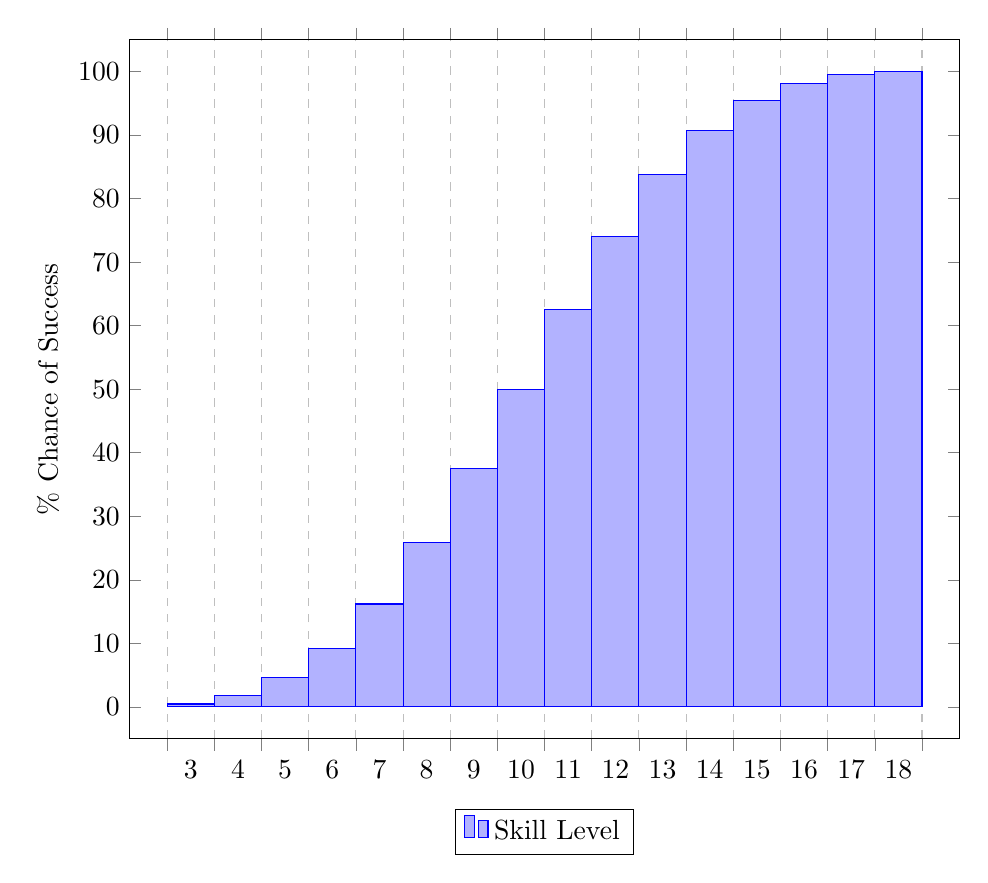
\begin{tikzpicture}
\begin{axis}[
	x tick label style={/pgf/number format/1000 sep=},
	ylabel=\% Chance of Success,
	enlargelimits=0.05,
	ytick = {0, 10, 20, 30, 40, 50, 60, 70, 80, 90, 100},
	legend style = {
	    at={(0.5,-0.1)},
	    grid style = dashed,
	    anchor=north,legend columns=-1
	},
	ybar interval = 1,
]
\addplot 
	coordinates {
	    (3,    0.46) 
	    (4,    1.85)
		(5,    4.63) 
		(6,    9.26) 
		(7,   16.20) 
		(8,   25.93) 
		(9,   37.50) 
		(10,  50.00) 
		(11,  62.50) 
		(12,  74.07)
		(13,  83.80)
		(14,  90.74)
		(15,  95.37)
		(16,  98.15)
		(17,  99.54)
		(18, 100.00)
		(19, 0)
	};
\legend{Skill Level}
\end{axis}
\end{tikzpicture}\\
The graph above shows the probability of succeeding a skill roll. If your character has an effective skill of 10, they have a 50\% chance of succeeding that roll. If they have a skill of 12, the chance of success goes up to 74\%.
\section{Critical Miss Table (Melee)}
\begin{center}
\begin{tabular}{r | l}
    \textbf{Roll} & \textbf{Result}\\\hline
    1 & Your weapon turns in your hand, and you hit with the flat side! \\
    2 & Your weapon breaks! \\
    3 & You lose your grip and the weapon flies out of your hand! \\
    4 & You lose your balance, and your turn! \\
    5 & You trip and fall! You have to get up again.\\
    6 & You hit yourself in the arm or leg! (50\% chance of hitting either)\\
\end{tabular}
\end{center}
\paragraph{Note}For \#3, the weapon flies 1d6 squares (50\% chance forward or backward). If it hits someone, it does half damage and lands there.

%% \section{Critical Miss Table (Ranged)}
%% \begin{center}
%% \begin{tabular}{r | l}
%%     \textbf{Roll} & \textbf{Result}\\\hline
%%     1 & Your weapon jams.\\
%%     2 &\\
%%     3 &\\
%%     4 &\\
%%     5 &\\
%%     6 &\\
%% \end{tabular}
%% \end{center}

\section{Weapons} \label{sec:weapons}
\subsection{Melee Weapons}
\begin{center}
\begin{tabular}{c|c|c|c|c|c}
    \textbf{Category} & \textbf{Name} & \textbf{Class} & \textbf{Damage} & \textbf{Damage Type} & \textbf{Range} \\\hline
    Unarmed  & Fists          & Light & d6-2 & Crushing & Close/1\\
             & Feet           & Light & d6-1 & Crushing & Close/1\\\hline
    Medieval & Short Sword    & Light & d6   & Slashing & Close/1\\
             & Long Sword     & Heavy & d6+2 & Slashing & 1 to 2 \\
             & Mace           & Heavy & d6+2 & Crushing & Close/1\\\hline
    Modern   & Baseball Bat   & Heavy & d6+1 & Crushing & Close/1\\
             & Aluminium Bat  & Light & d6+1 & Crushing & Close/1\\
             & Brass Knuckles & Light & d6-1 & Crushing & Close/1\\\hline
    Future   & Beam Sword     & Light & d6+3 & Slashing & Close/1
\end{tabular}
\end{center}

\subsection{Ranged Weapons}
\begin{center}
\begin{tabular}{c|c|c|c|c}
    \textbf{Category} & \textbf{Name} & \textbf{Damage} & \textbf{Damage Type} & \textbf{Accurate Range} \\\hline
    Primitive & Rock        & d6-1  & Crushing & $0.5 \times Shooting + Prof$  \\\hline
    Medieval  & Short Bow   & d6+1  & Piercing & $Shooting + Prof$ \\
              & Long Bow    & d6+2  & Piercing & $2 \times Shooting + Prof$ \\\hline
    Modern    & Pistol      & 2d6+2 & Crushing & 56m \\
              & Shotgun     & 5d6   & Crushing & 3m \\\hline
    Future    & Laser Gun   & 6d6   & Piercing & 66m \\
\end{tabular}
\end{center}
\paragraph{Note} These ranges are for when you want to shoot without a range penalty.
So despite the fact that a pistol can shoot around 1800m, it's incredibly hard to do so.

\section{Armour}
\begin{center}
\begin{tabular}{c|c|c|c}
\textbf{Category} & \textbf{Name}  & \textbf{PD} & \textbf{DR}\\\hline
         Medieval & Learther       & 1 & 1 \\
                  & Half Plate     & 2 & 2 \\
                  & Full Plate     & 4 & 3 \\
                  & Chain Mail     & 1 & 1 \\\hline
           Modern & Summer Clothes & 0 & 0 \\
                  & Winter Clothes & 0 & 1 \\
                  & Kevlar Vest    & 1 & 3 \\\hline
           Future & Polymer        & 4 & 3 \\
\end{tabular}
\end{center}

\chapter{Character Sheets}\label{app:character-sheets}
This Appendix contains some example character sheets as well as an empty one ready for printout.
\includepdf[pages = -]{graphics/character-sheet-example.pdf}
\includepdf[pages = -]{graphics/siren-character-sheet.pdf}
\end{document}

\end{document}
